% Created by tikzDevice version 0.12.4 on 2023-06-18 13:02:28
% !TEX encoding = UTF-8 Unicode
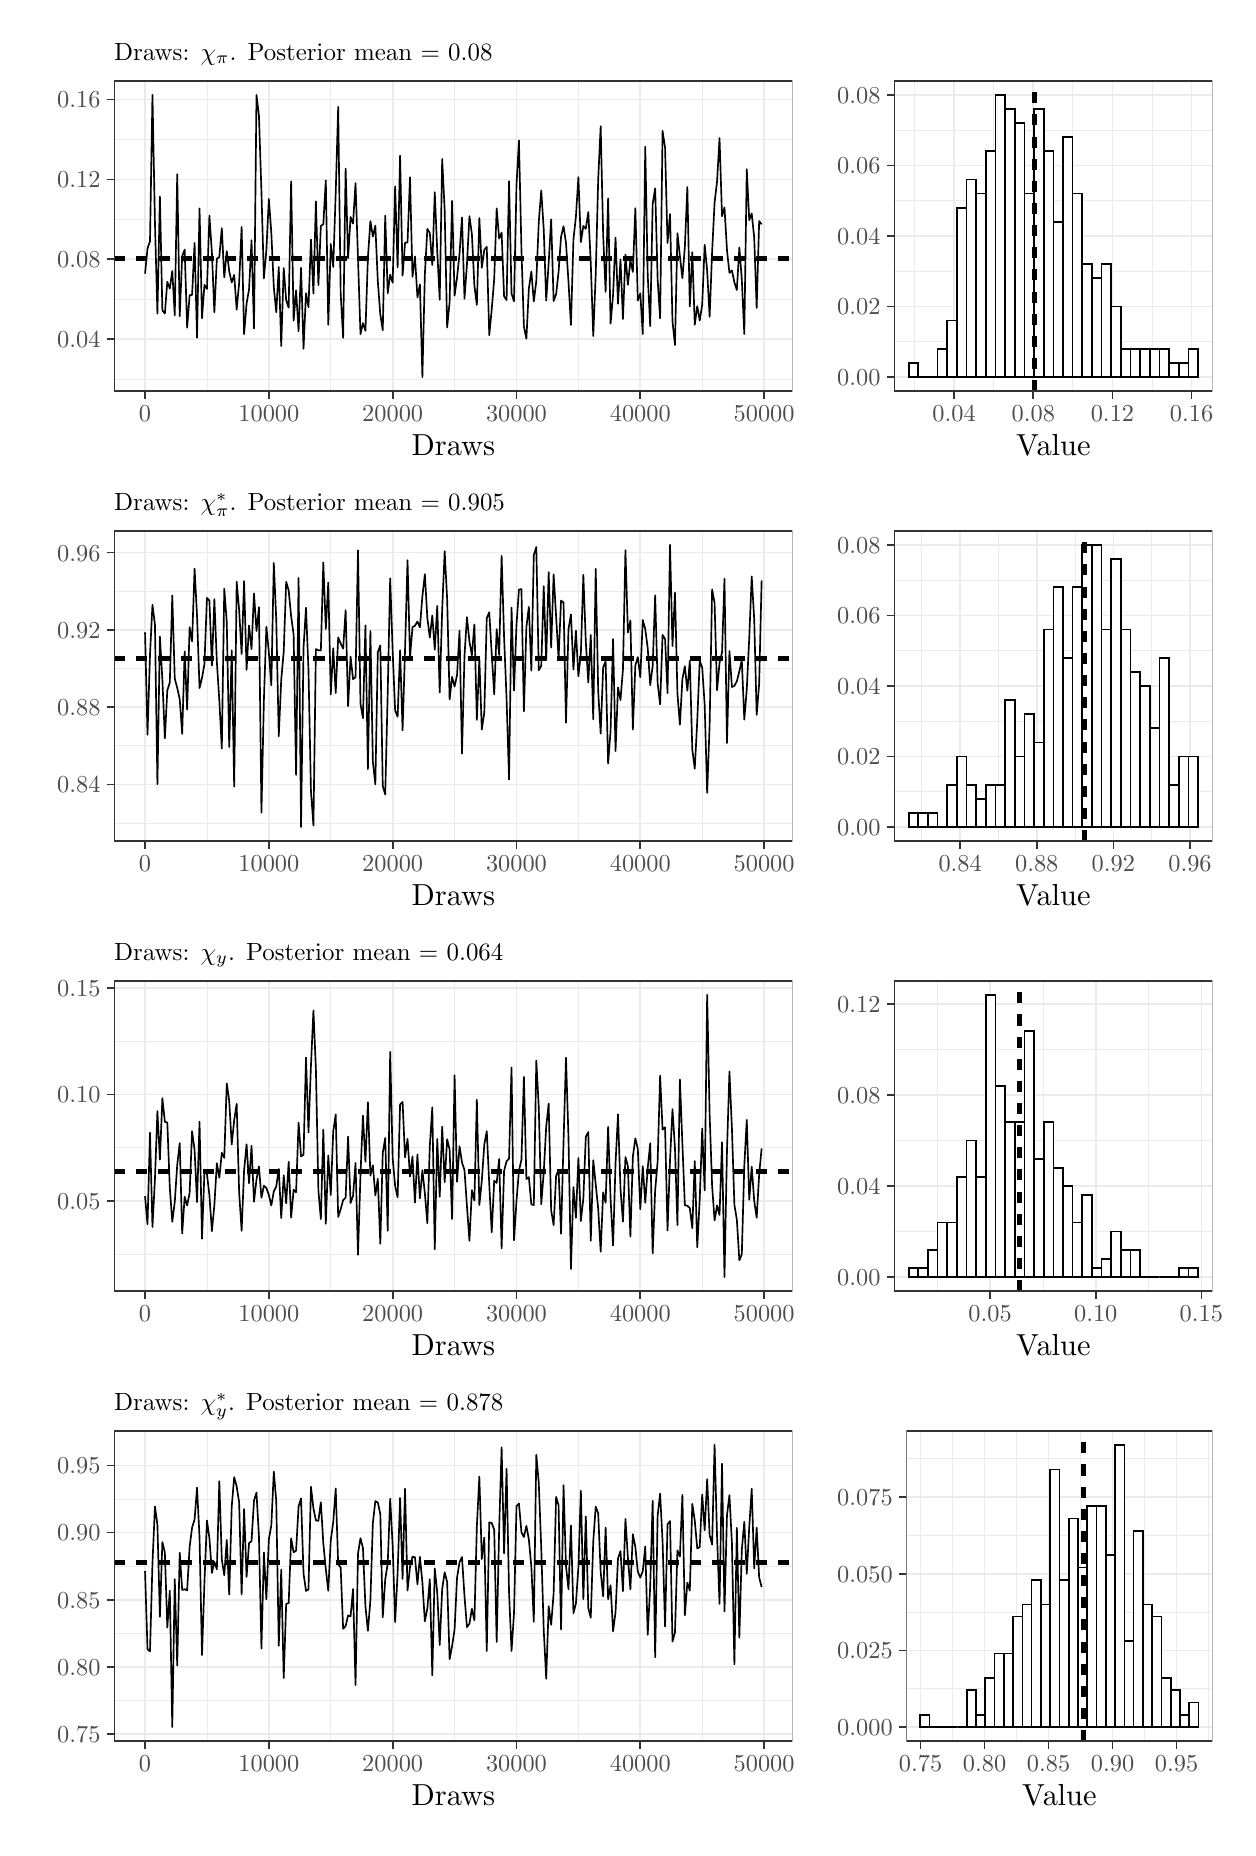
\begin{tikzpicture}[x=1pt,y=1pt]
\definecolor{fillColor}{RGB}{255,255,255}
\path[use as bounding box,fill=fillColor,fill opacity=0.00] (0,0) rectangle (433.62,650.43);
\begin{scope}
\path[clip] (  0.00,487.82) rectangle (281.85,650.43);
\definecolor{drawColor}{RGB}{255,255,255}
\definecolor{fillColor}{RGB}{255,255,255}

\path[draw=drawColor,line width= 0.6pt,line join=round,line cap=round,fill=fillColor] (  0.00,487.82) rectangle (281.85,650.43);
\end{scope}
\begin{scope}
\path[clip] ( 31.27,519.08) rectangle (276.35,631.24);
\definecolor{fillColor}{RGB}{255,255,255}

\path[fill=fillColor] ( 31.27,519.08) rectangle (276.35,631.24);
\definecolor{drawColor}{gray}{0.92}

\path[draw=drawColor,line width= 0.3pt,line join=round] ( 31.27,523.42) --
	(276.35,523.42);

\path[draw=drawColor,line width= 0.3pt,line join=round] ( 31.27,552.29) --
	(276.35,552.29);

\path[draw=drawColor,line width= 0.3pt,line join=round] ( 31.27,581.16) --
	(276.35,581.16);

\path[draw=drawColor,line width= 0.3pt,line join=round] ( 31.27,610.03) --
	(276.35,610.03);

\path[draw=drawColor,line width= 0.3pt,line join=round] ( 64.78,519.08) --
	( 64.78,631.24);

\path[draw=drawColor,line width= 0.3pt,line join=round] (109.52,519.08) --
	(109.52,631.24);

\path[draw=drawColor,line width= 0.3pt,line join=round] (154.26,519.08) --
	(154.26,631.24);

\path[draw=drawColor,line width= 0.3pt,line join=round] (199.00,519.08) --
	(199.00,631.24);

\path[draw=drawColor,line width= 0.3pt,line join=round] (243.74,519.08) --
	(243.74,631.24);

\path[draw=drawColor,line width= 0.6pt,line join=round] ( 31.27,537.86) --
	(276.35,537.86);

\path[draw=drawColor,line width= 0.6pt,line join=round] ( 31.27,566.73) --
	(276.35,566.73);

\path[draw=drawColor,line width= 0.6pt,line join=round] ( 31.27,595.60) --
	(276.35,595.60);

\path[draw=drawColor,line width= 0.6pt,line join=round] ( 31.27,624.47) --
	(276.35,624.47);

\path[draw=drawColor,line width= 0.6pt,line join=round] ( 42.41,519.08) --
	( 42.41,631.24);

\path[draw=drawColor,line width= 0.6pt,line join=round] ( 87.15,519.08) --
	( 87.15,631.24);

\path[draw=drawColor,line width= 0.6pt,line join=round] (131.89,519.08) --
	(131.89,631.24);

\path[draw=drawColor,line width= 0.6pt,line join=round] (176.63,519.08) --
	(176.63,631.24);

\path[draw=drawColor,line width= 0.6pt,line join=round] (221.37,519.08) --
	(221.37,631.24);

\path[draw=drawColor,line width= 0.6pt,line join=round] (266.11,519.08) --
	(266.11,631.24);
\definecolor{drawColor}{RGB}{0,0,0}

\path[draw=drawColor,line width= 0.6pt,line join=round] ( 42.41,561.56) --
	( 43.30,570.61) --
	( 44.20,573.27) --
	( 45.09,626.15) --
	( 45.99,580.05) --
	( 46.88,547.07) --
	( 47.78,589.42) --
	( 48.67,548.30) --
	( 49.57,547.12) --
	( 50.46,558.61) --
	( 51.36,556.11) --
	( 52.25,562.53) --
	( 53.15,546.47) --
	( 54.04,597.44) --
	( 54.94,546.11) --
	( 55.83,567.81) --
	( 56.73,570.22) --
	( 57.62,541.99) --
	( 58.52,553.73) --
	( 59.41,553.87) --
	( 60.31,572.62) --
	( 61.20,538.35) --
	( 62.10,585.13) --
	( 62.99,545.45) --
	( 63.88,557.50) --
	( 64.78,556.00) --
	( 65.67,582.49) --
	( 66.57,569.16) --
	( 67.46,547.55) --
	( 68.36,566.92) --
	( 69.25,567.56) --
	( 70.15,577.97) --
	( 71.04,560.20) --
	( 71.94,569.67) --
	( 72.83,562.41) --
	( 73.73,558.36) --
	( 74.62,561.07) --
	( 75.52,548.55) --
	( 76.41,558.16) --
	( 77.31,578.45) --
	( 78.20,539.66) --
	( 79.10,550.72) --
	( 79.99,555.84) --
	( 80.89,573.61) --
	( 81.78,541.68) --
	( 82.68,626.09) --
	( 83.57,618.63) --
	( 84.47,591.26) --
	( 85.36,559.84) --
	( 86.25,570.04) --
	( 87.15,588.52) --
	( 88.04,576.36) --
	( 88.94,556.65) --
	( 89.83,547.58) --
	( 90.73,563.92) --
	( 91.62,535.35) --
	( 92.52,563.55) --
	( 93.41,551.90) --
	( 94.31,549.25) --
	( 95.20,594.90) --
	( 96.10,544.55) --
	( 96.99,555.51) --
	( 97.89,540.72) --
	( 98.78,563.63) --
	( 99.68,534.39) --
	(100.57,554.48) --
	(101.47,549.41) --
	(102.36,573.86) --
	(103.26,554.32) --
	(104.15,587.67) --
	(105.05,557.39) --
	(105.94,578.76) --
	(106.83,579.42) --
	(107.73,595.27) --
	(108.62,543.08) --
	(109.52,572.27) --
	(110.41,563.95) --
	(111.31,590.84) --
	(112.20,621.80) --
	(113.10,554.40) --
	(113.99,538.32) --
	(114.89,599.52) --
	(115.78,567.12) --
	(116.68,582.03) --
	(117.57,579.64) --
	(118.47,594.25) --
	(119.36,567.16) --
	(120.26,539.67) --
	(121.15,543.65) --
	(122.05,540.89) --
	(122.94,567.31) --
	(123.84,580.53) --
	(124.73,574.98) --
	(125.63,578.88) --
	(126.52,558.80) --
	(127.42,546.80) --
	(128.31,541.06) --
	(129.20,582.52) --
	(130.10,554.46) --
	(130.99,561.20) --
	(131.89,558.26) --
	(132.78,593.06) --
	(133.68,563.78) --
	(134.57,604.18) --
	(135.47,560.87) --
	(136.36,572.66) --
	(137.26,572.86) --
	(138.15,596.35) --
	(139.05,560.41) --
	(139.94,567.73) --
	(140.84,552.95) --
	(141.73,557.66) --
	(142.63,524.17) --
	(143.52,561.20) --
	(144.42,577.71) --
	(145.31,576.25) --
	(146.21,564.63) --
	(147.10,590.96) --
	(148.00,569.56) --
	(148.89,552.11) --
	(149.78,602.97) --
	(150.68,584.40) --
	(151.57,542.07) --
	(152.47,551.24) --
	(153.36,587.87) --
	(154.26,553.57) --
	(155.15,560.11) --
	(156.05,568.78) --
	(156.94,581.87) --
	(157.84,552.47) --
	(158.73,564.90) --
	(159.63,582.32) --
	(160.52,575.78) --
	(161.42,557.23) --
	(162.31,550.21) --
	(163.21,581.63) --
	(164.10,563.64) --
	(165.00,570.14) --
	(165.89,571.25) --
	(166.79,539.27) --
	(167.68,548.55) --
	(168.58,559.61) --
	(169.47,585.13) --
	(170.37,574.22) --
	(171.26,576.36) --
	(172.15,553.34) --
	(173.05,552.00) --
	(173.94,594.92) --
	(174.84,554.36) --
	(175.73,551.56) --
	(176.63,593.52) --
	(177.52,609.68) --
	(178.42,570.36) --
	(179.31,542.43) --
	(180.21,538.03) --
	(181.10,556.16) --
	(182.00,562.29) --
	(182.89,551.49) --
	(183.79,558.82) --
	(184.68,580.15) --
	(185.58,591.62) --
	(186.47,577.64) --
	(187.37,551.78) --
	(188.26,565.40) --
	(189.16,581.17) --
	(190.05,551.64) --
	(190.95,554.12) --
	(191.84,562.19) --
	(192.73,574.82) --
	(193.63,578.67) --
	(194.52,572.62) --
	(195.42,558.60) --
	(196.31,542.96) --
	(197.21,573.95) --
	(198.10,582.04) --
	(199.00,596.42) --
	(199.89,572.93) --
	(200.79,578.80) --
	(201.68,577.71) --
	(202.58,583.79) --
	(203.47,565.47) --
	(204.37,539.03) --
	(205.26,561.21) --
	(206.16,595.63) --
	(207.05,614.81) --
	(207.95,575.57) --
	(208.84,554.97) --
	(209.74,588.74) --
	(210.63,543.47) --
	(211.53,553.84) --
	(212.42,574.57) --
	(213.31,550.64) --
	(214.21,566.65) --
	(215.10,545.15) --
	(216.00,568.41) --
	(216.89,557.52) --
	(217.79,566.40) --
	(218.68,562.15) --
	(219.58,585.19) --
	(220.47,551.80) --
	(221.37,554.38) --
	(222.26,539.68) --
	(223.16,607.37) --
	(224.05,560.92) --
	(224.95,542.57) --
	(225.84,586.73) --
	(226.74,592.38) --
	(227.63,559.57) --
	(228.53,545.37) --
	(229.42,613.13) --
	(230.32,607.01) --
	(231.21,572.60) --
	(232.11,583.06) --
	(233.00,544.27) --
	(233.90,535.76) --
	(234.79,576.14) --
	(235.68,567.85) --
	(236.58,559.89) --
	(237.47,571.19) --
	(238.37,592.84) --
	(239.26,549.68) --
	(240.16,569.27) --
	(241.05,543.08) --
	(241.95,549.78) --
	(242.84,544.59) --
	(243.74,550.38) --
	(244.63,571.95) --
	(245.53,562.64) --
	(246.42,545.90) --
	(247.32,569.41) --
	(248.21,587.23) --
	(249.11,594.88) --
	(250.00,610.53) --
	(250.90,582.29) --
	(251.79,585.47) --
	(252.69,570.07) --
	(253.58,561.79) --
	(254.48,562.69) --
	(255.37,558.41) --
	(256.26,555.62) --
	(257.16,571.00) --
	(258.05,559.42) --
	(258.95,539.70) --
	(259.84,599.28) --
	(260.74,580.86) --
	(261.63,583.27) --
	(262.53,574.57) --
	(263.42,549.14) --
	(264.32,580.54) --
	(265.21,579.36);

\path[draw=drawColor,line width= 1.7pt,dash pattern=on 4pt off 4pt ,line join=round] ( 31.27,567.08) -- (276.35,567.08);
\definecolor{drawColor}{gray}{0.20}

\path[draw=drawColor,line width= 0.6pt,line join=round,line cap=round] ( 31.27,519.08) rectangle (276.35,631.24);
\end{scope}
\begin{scope}
\path[clip] (  0.00,  0.00) rectangle (433.62,650.43);
\definecolor{drawColor}{gray}{0.30}

\node[text=drawColor,anchor=base east,inner sep=0pt, outer sep=0pt, scale=  0.88] at ( 26.32,534.83) {0.04};

\node[text=drawColor,anchor=base east,inner sep=0pt, outer sep=0pt, scale=  0.88] at ( 26.32,563.70) {0.08};

\node[text=drawColor,anchor=base east,inner sep=0pt, outer sep=0pt, scale=  0.88] at ( 26.32,592.57) {0.12};

\node[text=drawColor,anchor=base east,inner sep=0pt, outer sep=0pt, scale=  0.88] at ( 26.32,621.44) {0.16};
\end{scope}
\begin{scope}
\path[clip] (  0.00,  0.00) rectangle (433.62,650.43);
\definecolor{drawColor}{gray}{0.20}

\path[draw=drawColor,line width= 0.6pt,line join=round] ( 28.52,537.86) --
	( 31.27,537.86);

\path[draw=drawColor,line width= 0.6pt,line join=round] ( 28.52,566.73) --
	( 31.27,566.73);

\path[draw=drawColor,line width= 0.6pt,line join=round] ( 28.52,595.60) --
	( 31.27,595.60);

\path[draw=drawColor,line width= 0.6pt,line join=round] ( 28.52,624.47) --
	( 31.27,624.47);
\end{scope}
\begin{scope}
\path[clip] (  0.00,  0.00) rectangle (433.62,650.43);
\definecolor{drawColor}{gray}{0.20}

\path[draw=drawColor,line width= 0.6pt,line join=round] ( 42.41,516.33) --
	( 42.41,519.08);

\path[draw=drawColor,line width= 0.6pt,line join=round] ( 87.15,516.33) --
	( 87.15,519.08);

\path[draw=drawColor,line width= 0.6pt,line join=round] (131.89,516.33) --
	(131.89,519.08);

\path[draw=drawColor,line width= 0.6pt,line join=round] (176.63,516.33) --
	(176.63,519.08);

\path[draw=drawColor,line width= 0.6pt,line join=round] (221.37,516.33) --
	(221.37,519.08);

\path[draw=drawColor,line width= 0.6pt,line join=round] (266.11,516.33) --
	(266.11,519.08);
\end{scope}
\begin{scope}
\path[clip] (  0.00,  0.00) rectangle (433.62,650.43);
\definecolor{drawColor}{gray}{0.30}

\node[text=drawColor,anchor=base,inner sep=0pt, outer sep=0pt, scale=  0.88] at ( 42.41,508.06) {0};

\node[text=drawColor,anchor=base,inner sep=0pt, outer sep=0pt, scale=  0.88] at ( 87.15,508.06) {10000};

\node[text=drawColor,anchor=base,inner sep=0pt, outer sep=0pt, scale=  0.88] at (131.89,508.06) {20000};

\node[text=drawColor,anchor=base,inner sep=0pt, outer sep=0pt, scale=  0.88] at (176.63,508.06) {30000};

\node[text=drawColor,anchor=base,inner sep=0pt, outer sep=0pt, scale=  0.88] at (221.37,508.06) {40000};

\node[text=drawColor,anchor=base,inner sep=0pt, outer sep=0pt, scale=  0.88] at (266.11,508.06) {50000};
\end{scope}
\begin{scope}
\path[clip] (  0.00,  0.00) rectangle (433.62,650.43);
\definecolor{drawColor}{RGB}{0,0,0}

\node[text=drawColor,anchor=base,inner sep=0pt, outer sep=0pt, scale=  1.10] at (153.81,495.75) {Draws};
\end{scope}
\begin{scope}
\path[clip] (  0.00,  0.00) rectangle (433.62,650.43);
\definecolor{drawColor}{RGB}{0,0,0}

\node[text=drawColor,anchor=base west,inner sep=0pt, outer sep=0pt, scale=  0.90] at ( 31.27,638.73) {Draws: $\chi_{\pi}$. Posterior mean = 0.08};
\end{scope}
\begin{scope}
\path[clip] (281.85,487.82) rectangle (433.62,650.43);
\definecolor{drawColor}{RGB}{255,255,255}
\definecolor{fillColor}{RGB}{255,255,255}

\path[draw=drawColor,line width= 0.6pt,line join=round,line cap=round,fill=fillColor] (281.85,487.82) rectangle (433.62,650.43);
\end{scope}
\begin{scope}
\path[clip] (313.12,519.08) rectangle (428.12,631.24);
\definecolor{fillColor}{RGB}{255,255,255}

\path[fill=fillColor] (313.12,519.08) rectangle (428.12,631.24);
\definecolor{drawColor}{gray}{0.92}

\path[draw=drawColor,line width= 0.3pt,line join=round] (313.12,536.92) --
	(428.12,536.92);

\path[draw=drawColor,line width= 0.3pt,line join=round] (313.12,562.41) --
	(428.12,562.41);

\path[draw=drawColor,line width= 0.3pt,line join=round] (313.12,587.91) --
	(428.12,587.91);

\path[draw=drawColor,line width= 0.3pt,line join=round] (313.12,613.40) --
	(428.12,613.40);

\path[draw=drawColor,line width= 0.3pt,line join=round] (320.46,519.08) --
	(320.46,631.24);

\path[draw=drawColor,line width= 0.3pt,line join=round] (349.07,519.08) --
	(349.07,631.24);

\path[draw=drawColor,line width= 0.3pt,line join=round] (377.68,519.08) --
	(377.68,631.24);

\path[draw=drawColor,line width= 0.3pt,line join=round] (406.29,519.08) --
	(406.29,631.24);

\path[draw=drawColor,line width= 0.6pt,line join=round] (313.12,524.17) --
	(428.12,524.17);

\path[draw=drawColor,line width= 0.6pt,line join=round] (313.12,549.67) --
	(428.12,549.67);

\path[draw=drawColor,line width= 0.6pt,line join=round] (313.12,575.16) --
	(428.12,575.16);

\path[draw=drawColor,line width= 0.6pt,line join=round] (313.12,600.65) --
	(428.12,600.65);

\path[draw=drawColor,line width= 0.6pt,line join=round] (313.12,626.15) --
	(428.12,626.15);

\path[draw=drawColor,line width= 0.6pt,line join=round] (334.76,519.08) --
	(334.76,631.24);

\path[draw=drawColor,line width= 0.6pt,line join=round] (363.38,519.08) --
	(363.38,631.24);

\path[draw=drawColor,line width= 0.6pt,line join=round] (391.99,519.08) --
	(391.99,631.24);

\path[draw=drawColor,line width= 0.6pt,line join=round] (420.60,519.08) --
	(420.60,631.24);
\definecolor{drawColor}{RGB}{0,0,0}

\path[draw=drawColor,line width= 0.6pt,fill=fillColor] (318.35,524.17) rectangle (321.83,529.27);

\path[draw=drawColor,line width= 0.6pt,fill=fillColor] (321.83,524.17) rectangle (325.32,524.17);

\path[draw=drawColor,line width= 0.6pt,fill=fillColor] (325.32,524.17) rectangle (328.80,524.17);

\path[draw=drawColor,line width= 0.6pt,fill=fillColor] (328.80,524.17) rectangle (332.29,534.37);

\path[draw=drawColor,line width= 0.6pt,fill=fillColor] (332.29,524.17) rectangle (335.77,544.57);

\path[draw=drawColor,line width= 0.6pt,fill=fillColor] (335.77,524.17) rectangle (339.26,585.36);

\path[draw=drawColor,line width= 0.6pt,fill=fillColor] (339.26,524.17) rectangle (342.74,595.55);

\path[draw=drawColor,line width= 0.6pt,fill=fillColor] (342.74,524.17) rectangle (346.23,590.46);

\path[draw=drawColor,line width= 0.6pt,fill=fillColor] (346.23,524.17) rectangle (349.71,605.75);

\path[draw=drawColor,line width= 0.6pt,fill=fillColor] (349.71,524.17) rectangle (353.20,626.15);

\path[draw=drawColor,line width= 0.6pt,fill=fillColor] (353.20,524.17) rectangle (356.68,621.05);

\path[draw=drawColor,line width= 0.6pt,fill=fillColor] (356.68,524.17) rectangle (360.17,615.95);

\path[draw=drawColor,line width= 0.6pt,fill=fillColor] (360.17,524.17) rectangle (363.65,590.46);

\path[draw=drawColor,line width= 0.6pt,fill=fillColor] (363.65,524.17) rectangle (367.14,621.05);

\path[draw=drawColor,line width= 0.6pt,fill=fillColor] (367.14,524.17) rectangle (370.62,605.75);

\path[draw=drawColor,line width= 0.6pt,fill=fillColor] (370.62,524.17) rectangle (374.11,580.26);

\path[draw=drawColor,line width= 0.6pt,fill=fillColor] (374.11,524.17) rectangle (377.59,610.85);

\path[draw=drawColor,line width= 0.6pt,fill=fillColor] (377.59,524.17) rectangle (381.08,590.46);

\path[draw=drawColor,line width= 0.6pt,fill=fillColor] (381.08,524.17) rectangle (384.56,564.96);

\path[draw=drawColor,line width= 0.6pt,fill=fillColor] (384.56,524.17) rectangle (388.05,559.86);

\path[draw=drawColor,line width= 0.6pt,fill=fillColor] (388.05,524.17) rectangle (391.53,564.96);

\path[draw=drawColor,line width= 0.6pt,fill=fillColor] (391.53,524.17) rectangle (395.01,549.67);

\path[draw=drawColor,line width= 0.6pt,fill=fillColor] (395.01,524.17) rectangle (398.50,534.37);

\path[draw=drawColor,line width= 0.6pt,fill=fillColor] (398.50,524.17) rectangle (401.98,534.37);

\path[draw=drawColor,line width= 0.6pt,fill=fillColor] (401.98,524.17) rectangle (405.47,534.37);

\path[draw=drawColor,line width= 0.6pt,fill=fillColor] (405.47,524.17) rectangle (408.95,534.37);

\path[draw=drawColor,line width= 0.6pt,fill=fillColor] (408.95,524.17) rectangle (412.44,534.37);

\path[draw=drawColor,line width= 0.6pt,fill=fillColor] (412.44,524.17) rectangle (415.92,529.27);

\path[draw=drawColor,line width= 0.6pt,fill=fillColor] (415.92,524.17) rectangle (419.41,529.27);

\path[draw=drawColor,line width= 0.6pt,fill=fillColor] (419.41,524.17) rectangle (422.89,534.37);

\path[draw=drawColor,line width= 1.7pt,dash pattern=on 4pt off 4pt ,line join=round] (363.73,519.08) -- (363.73,631.24);
\definecolor{drawColor}{gray}{0.20}

\path[draw=drawColor,line width= 0.6pt,line join=round,line cap=round] (313.12,519.08) rectangle (428.12,631.24);
\end{scope}
\begin{scope}
\path[clip] (  0.00,  0.00) rectangle (433.62,650.43);
\definecolor{drawColor}{gray}{0.30}

\node[text=drawColor,anchor=base east,inner sep=0pt, outer sep=0pt, scale=  0.88] at (308.17,521.14) {0.00};

\node[text=drawColor,anchor=base east,inner sep=0pt, outer sep=0pt, scale=  0.88] at (308.17,546.64) {0.02};

\node[text=drawColor,anchor=base east,inner sep=0pt, outer sep=0pt, scale=  0.88] at (308.17,572.13) {0.04};

\node[text=drawColor,anchor=base east,inner sep=0pt, outer sep=0pt, scale=  0.88] at (308.17,597.62) {0.06};

\node[text=drawColor,anchor=base east,inner sep=0pt, outer sep=0pt, scale=  0.88] at (308.17,623.12) {0.08};
\end{scope}
\begin{scope}
\path[clip] (  0.00,  0.00) rectangle (433.62,650.43);
\definecolor{drawColor}{gray}{0.20}

\path[draw=drawColor,line width= 0.6pt,line join=round] (310.37,524.17) --
	(313.12,524.17);

\path[draw=drawColor,line width= 0.6pt,line join=round] (310.37,549.67) --
	(313.12,549.67);

\path[draw=drawColor,line width= 0.6pt,line join=round] (310.37,575.16) --
	(313.12,575.16);

\path[draw=drawColor,line width= 0.6pt,line join=round] (310.37,600.65) --
	(313.12,600.65);

\path[draw=drawColor,line width= 0.6pt,line join=round] (310.37,626.15) --
	(313.12,626.15);
\end{scope}
\begin{scope}
\path[clip] (  0.00,  0.00) rectangle (433.62,650.43);
\definecolor{drawColor}{gray}{0.20}

\path[draw=drawColor,line width= 0.6pt,line join=round] (334.76,516.33) --
	(334.76,519.08);

\path[draw=drawColor,line width= 0.6pt,line join=round] (363.38,516.33) --
	(363.38,519.08);

\path[draw=drawColor,line width= 0.6pt,line join=round] (391.99,516.33) --
	(391.99,519.08);

\path[draw=drawColor,line width= 0.6pt,line join=round] (420.60,516.33) --
	(420.60,519.08);
\end{scope}
\begin{scope}
\path[clip] (  0.00,  0.00) rectangle (433.62,650.43);
\definecolor{drawColor}{gray}{0.30}

\node[text=drawColor,anchor=base,inner sep=0pt, outer sep=0pt, scale=  0.88] at (334.76,508.06) {0.04};

\node[text=drawColor,anchor=base,inner sep=0pt, outer sep=0pt, scale=  0.88] at (363.38,508.06) {0.08};

\node[text=drawColor,anchor=base,inner sep=0pt, outer sep=0pt, scale=  0.88] at (391.99,508.06) {0.12};

\node[text=drawColor,anchor=base,inner sep=0pt, outer sep=0pt, scale=  0.88] at (420.60,508.06) {0.16};
\end{scope}
\begin{scope}
\path[clip] (  0.00,  0.00) rectangle (433.62,650.43);
\definecolor{drawColor}{RGB}{0,0,0}

\node[text=drawColor,anchor=base,inner sep=0pt, outer sep=0pt, scale=  1.10] at (370.62,495.75) {Value};
\end{scope}
\begin{scope}
\path[clip] (  0.00,325.21) rectangle (281.85,487.82);
\definecolor{drawColor}{RGB}{255,255,255}
\definecolor{fillColor}{RGB}{255,255,255}

\path[draw=drawColor,line width= 0.6pt,line join=round,line cap=round,fill=fillColor] (  0.00,325.21) rectangle (281.85,487.82);
\end{scope}
\begin{scope}
\path[clip] ( 31.27,356.47) rectangle (276.35,468.64);
\definecolor{fillColor}{RGB}{255,255,255}

\path[fill=fillColor] ( 31.27,356.47) rectangle (276.35,468.64);
\definecolor{drawColor}{gray}{0.92}

\path[draw=drawColor,line width= 0.3pt,line join=round] ( 31.27,362.96) --
	(276.35,362.96);

\path[draw=drawColor,line width= 0.3pt,line join=round] ( 31.27,390.90) --
	(276.35,390.90);

\path[draw=drawColor,line width= 0.3pt,line join=round] ( 31.27,418.83) --
	(276.35,418.83);

\path[draw=drawColor,line width= 0.3pt,line join=round] ( 31.27,446.77) --
	(276.35,446.77);

\path[draw=drawColor,line width= 0.3pt,line join=round] ( 64.78,356.47) --
	( 64.78,468.64);

\path[draw=drawColor,line width= 0.3pt,line join=round] (109.52,356.47) --
	(109.52,468.64);

\path[draw=drawColor,line width= 0.3pt,line join=round] (154.26,356.47) --
	(154.26,468.64);

\path[draw=drawColor,line width= 0.3pt,line join=round] (199.00,356.47) --
	(199.00,468.64);

\path[draw=drawColor,line width= 0.3pt,line join=round] (243.74,356.47) --
	(243.74,468.64);

\path[draw=drawColor,line width= 0.6pt,line join=round] ( 31.27,376.93) --
	(276.35,376.93);

\path[draw=drawColor,line width= 0.6pt,line join=round] ( 31.27,404.87) --
	(276.35,404.87);

\path[draw=drawColor,line width= 0.6pt,line join=round] ( 31.27,432.80) --
	(276.35,432.80);

\path[draw=drawColor,line width= 0.6pt,line join=round] ( 31.27,460.74) --
	(276.35,460.74);

\path[draw=drawColor,line width= 0.6pt,line join=round] ( 42.41,356.47) --
	( 42.41,468.64);

\path[draw=drawColor,line width= 0.6pt,line join=round] ( 87.15,356.47) --
	( 87.15,468.64);

\path[draw=drawColor,line width= 0.6pt,line join=round] (131.89,356.47) --
	(131.89,468.64);

\path[draw=drawColor,line width= 0.6pt,line join=round] (176.63,356.47) --
	(176.63,468.64);

\path[draw=drawColor,line width= 0.6pt,line join=round] (221.37,356.47) --
	(221.37,468.64);

\path[draw=drawColor,line width= 0.6pt,line join=round] (266.11,356.47) --
	(266.11,468.64);
\definecolor{drawColor}{RGB}{0,0,0}

\path[draw=drawColor,line width= 0.6pt,line join=round] ( 42.41,431.95) --
	( 43.30,394.91) --
	( 44.20,423.77) --
	( 45.09,441.88) --
	( 45.99,434.70) --
	( 46.88,377.04) --
	( 47.78,430.37) --
	( 48.67,414.98) --
	( 49.57,393.61) --
	( 50.46,410.99) --
	( 51.36,413.78) --
	( 52.25,445.25) --
	( 53.15,415.20) --
	( 54.04,411.88) --
	( 54.94,407.72) --
	( 55.83,395.23) --
	( 56.73,425.01) --
	( 57.62,404.01) --
	( 58.52,433.80) --
	( 59.41,428.65) --
	( 60.31,454.94) --
	( 61.20,437.83) --
	( 62.10,411.79) --
	( 62.99,415.43) --
	( 63.88,420.49) --
	( 64.78,444.37) --
	( 65.67,443.41) --
	( 66.57,419.90) --
	( 67.46,443.91) --
	( 68.36,421.26) --
	( 69.25,407.37) --
	( 70.15,389.95) --
	( 71.04,447.70) --
	( 71.94,435.67) --
	( 72.83,390.46) --
	( 73.73,425.42) --
	( 74.62,376.18) --
	( 75.52,450.21) --
	( 76.41,440.08) --
	( 77.31,424.09) --
	( 78.20,450.43) --
	( 79.10,418.36) --
	( 79.99,434.41) --
	( 80.89,425.84) --
	( 81.78,446.00) --
	( 82.68,432.41) --
	( 83.57,440.98) --
	( 84.47,366.76) --
	( 85.36,407.52) --
	( 86.25,434.00) --
	( 87.15,424.63) --
	( 88.04,412.81) --
	( 88.94,456.98) --
	( 89.83,436.39) --
	( 90.73,394.39) --
	( 91.62,414.76) --
	( 92.52,424.93) --
	( 93.41,450.19) --
	( 94.31,447.10) --
	( 95.20,437.76) --
	( 96.10,431.12) --
	( 96.99,380.42) --
	( 97.89,451.58) --
	( 98.78,361.57) --
	( 99.68,426.29) --
	(100.57,440.84) --
	(101.47,418.31) --
	(102.36,374.54) --
	(103.26,362.13) --
	(104.15,425.89) --
	(105.05,425.45) --
	(105.94,425.39) --
	(106.83,457.16) --
	(107.73,433.12) --
	(108.62,449.91) --
	(109.52,409.46) --
	(110.41,426.21) --
	(111.31,409.99) --
	(112.20,430.12) --
	(113.10,427.90) --
	(113.99,426.02) --
	(114.89,439.94) --
	(115.78,405.26) --
	(116.68,423.14) --
	(117.57,415.00) --
	(118.47,415.73) --
	(119.36,461.56) --
	(120.26,406.14) --
	(121.15,400.88) --
	(122.05,434.44) --
	(122.94,382.50) --
	(123.84,432.42) --
	(124.73,385.22) --
	(125.63,377.00) --
	(126.52,424.71) --
	(127.42,427.20) --
	(128.31,376.39) --
	(129.20,373.35) --
	(130.10,410.18) --
	(130.99,451.46) --
	(131.89,424.98) --
	(132.78,403.71) --
	(133.68,401.44) --
	(134.57,425.44) --
	(135.47,396.49) --
	(136.36,425.59) --
	(137.26,458.01) --
	(138.15,422.77) --
	(139.05,433.81) --
	(139.94,434.30) --
	(140.84,435.85) --
	(141.73,433.71) --
	(142.63,444.96) --
	(143.52,452.96) --
	(144.42,437.16) --
	(145.31,430.04) --
	(146.21,438.00) --
	(147.10,425.66) --
	(148.00,441.47) --
	(148.89,410.20) --
	(149.78,440.08) --
	(150.68,461.23) --
	(151.57,444.03) --
	(152.47,407.71) --
	(153.36,415.84) --
	(154.26,412.32) --
	(155.15,416.46) --
	(156.05,432.50) --
	(156.94,388.16) --
	(157.84,423.40) --
	(158.73,437.43) --
	(159.63,428.59) --
	(160.52,423.62) --
	(161.42,434.78) --
	(162.31,400.29) --
	(163.21,422.39) --
	(164.10,396.79) --
	(165.00,403.00) --
	(165.89,437.10) --
	(166.79,439.19) --
	(167.68,424.25) --
	(168.58,409.51) --
	(169.47,433.05) --
	(170.37,423.73) --
	(171.26,459.55) --
	(172.15,430.23) --
	(173.05,407.88) --
	(173.94,378.77) --
	(174.84,440.86) --
	(175.73,410.91) --
	(176.63,434.60) --
	(177.52,447.39) --
	(178.42,447.55) --
	(179.31,403.38) --
	(180.21,433.81) --
	(181.10,441.12) --
	(182.00,418.10) --
	(182.89,459.88) --
	(183.79,462.74) --
	(184.68,418.23) --
	(185.58,419.76) --
	(186.47,448.58) --
	(187.37,421.93) --
	(188.26,453.67) --
	(189.16,426.42) --
	(190.05,452.90) --
	(190.95,437.68) --
	(191.84,422.48) --
	(192.73,443.37) --
	(193.63,442.75) --
	(194.52,399.24) --
	(195.42,433.03) --
	(196.31,438.41) --
	(197.21,418.45) --
	(198.10,432.51) --
	(199.00,416.05) --
	(199.89,424.29) --
	(200.79,452.69) --
	(201.68,428.45) --
	(202.58,413.80) --
	(203.47,430.97) --
	(204.37,400.54) --
	(205.26,454.88) --
	(206.16,410.61) --
	(207.05,395.33) --
	(207.95,419.30) --
	(208.84,421.39) --
	(209.74,384.52) --
	(210.63,396.38) --
	(211.53,429.51) --
	(212.42,389.01) --
	(213.31,412.03) --
	(214.21,407.46) --
	(215.10,418.55) --
	(216.00,461.62) --
	(216.89,431.86) --
	(217.79,436.26) --
	(218.68,396.77) --
	(219.58,419.98) --
	(220.47,422.98) --
	(221.37,415.70) --
	(222.26,436.39) --
	(223.16,433.12) --
	(224.05,426.27) --
	(224.95,412.83) --
	(225.84,419.74) --
	(226.74,445.31) --
	(227.63,413.58) --
	(228.53,405.85) --
	(229.42,430.98) --
	(230.32,429.52) --
	(231.21,409.95) --
	(232.11,463.54) --
	(233.00,426.99) --
	(233.90,446.26) --
	(234.79,409.83) --
	(235.68,398.58) --
	(236.58,414.98) --
	(237.47,419.68) --
	(238.37,410.85) --
	(239.26,421.59) --
	(240.16,389.54) --
	(241.05,382.66) --
	(241.95,399.97) --
	(242.84,421.59) --
	(243.74,419.21) --
	(244.63,405.74) --
	(245.53,373.93) --
	(246.42,398.34) --
	(247.32,447.44) --
	(248.21,442.53) --
	(249.11,411.01) --
	(250.00,420.86) --
	(250.90,424.66) --
	(251.79,451.32) --
	(252.69,391.93) --
	(253.58,425.16) --
	(254.48,412.17) --
	(255.37,412.58) --
	(256.26,414.25) --
	(257.16,417.87) --
	(258.05,421.88) --
	(258.95,400.38) --
	(259.84,411.27) --
	(260.74,430.01) --
	(261.63,452.12) --
	(262.53,436.69) --
	(263.42,402.09) --
	(264.32,413.43) --
	(265.21,450.73);

\path[draw=drawColor,line width= 1.7pt,dash pattern=on 4pt off 4pt ,line join=round] ( 31.27,422.38) -- (276.35,422.38);
\definecolor{drawColor}{gray}{0.20}

\path[draw=drawColor,line width= 0.6pt,line join=round,line cap=round] ( 31.27,356.47) rectangle (276.35,468.64);
\end{scope}
\begin{scope}
\path[clip] (  0.00,  0.00) rectangle (433.62,650.43);
\definecolor{drawColor}{gray}{0.30}

\node[text=drawColor,anchor=base east,inner sep=0pt, outer sep=0pt, scale=  0.88] at ( 26.32,373.90) {0.84};

\node[text=drawColor,anchor=base east,inner sep=0pt, outer sep=0pt, scale=  0.88] at ( 26.32,401.84) {0.88};

\node[text=drawColor,anchor=base east,inner sep=0pt, outer sep=0pt, scale=  0.88] at ( 26.32,429.77) {0.92};

\node[text=drawColor,anchor=base east,inner sep=0pt, outer sep=0pt, scale=  0.88] at ( 26.32,457.71) {0.96};
\end{scope}
\begin{scope}
\path[clip] (  0.00,  0.00) rectangle (433.62,650.43);
\definecolor{drawColor}{gray}{0.20}

\path[draw=drawColor,line width= 0.6pt,line join=round] ( 28.52,376.93) --
	( 31.27,376.93);

\path[draw=drawColor,line width= 0.6pt,line join=round] ( 28.52,404.87) --
	( 31.27,404.87);

\path[draw=drawColor,line width= 0.6pt,line join=round] ( 28.52,432.80) --
	( 31.27,432.80);

\path[draw=drawColor,line width= 0.6pt,line join=round] ( 28.52,460.74) --
	( 31.27,460.74);
\end{scope}
\begin{scope}
\path[clip] (  0.00,  0.00) rectangle (433.62,650.43);
\definecolor{drawColor}{gray}{0.20}

\path[draw=drawColor,line width= 0.6pt,line join=round] ( 42.41,353.72) --
	( 42.41,356.47);

\path[draw=drawColor,line width= 0.6pt,line join=round] ( 87.15,353.72) --
	( 87.15,356.47);

\path[draw=drawColor,line width= 0.6pt,line join=round] (131.89,353.72) --
	(131.89,356.47);

\path[draw=drawColor,line width= 0.6pt,line join=round] (176.63,353.72) --
	(176.63,356.47);

\path[draw=drawColor,line width= 0.6pt,line join=round] (221.37,353.72) --
	(221.37,356.47);

\path[draw=drawColor,line width= 0.6pt,line join=round] (266.11,353.72) --
	(266.11,356.47);
\end{scope}
\begin{scope}
\path[clip] (  0.00,  0.00) rectangle (433.62,650.43);
\definecolor{drawColor}{gray}{0.30}

\node[text=drawColor,anchor=base,inner sep=0pt, outer sep=0pt, scale=  0.88] at ( 42.41,345.46) {0};

\node[text=drawColor,anchor=base,inner sep=0pt, outer sep=0pt, scale=  0.88] at ( 87.15,345.46) {10000};

\node[text=drawColor,anchor=base,inner sep=0pt, outer sep=0pt, scale=  0.88] at (131.89,345.46) {20000};

\node[text=drawColor,anchor=base,inner sep=0pt, outer sep=0pt, scale=  0.88] at (176.63,345.46) {30000};

\node[text=drawColor,anchor=base,inner sep=0pt, outer sep=0pt, scale=  0.88] at (221.37,345.46) {40000};

\node[text=drawColor,anchor=base,inner sep=0pt, outer sep=0pt, scale=  0.88] at (266.11,345.46) {50000};
\end{scope}
\begin{scope}
\path[clip] (  0.00,  0.00) rectangle (433.62,650.43);
\definecolor{drawColor}{RGB}{0,0,0}

\node[text=drawColor,anchor=base,inner sep=0pt, outer sep=0pt, scale=  1.10] at (153.81,333.14) {Draws};
\end{scope}
\begin{scope}
\path[clip] (  0.00,  0.00) rectangle (433.62,650.43);
\definecolor{drawColor}{RGB}{0,0,0}

\node[text=drawColor,anchor=base west,inner sep=0pt, outer sep=0pt, scale=  0.90] at ( 31.27,476.12) {Draws: $\chi^*_{\pi}$. Posterior mean = 0.905};
\end{scope}
\begin{scope}
\path[clip] (281.85,325.21) rectangle (433.62,487.82);
\definecolor{drawColor}{RGB}{255,255,255}
\definecolor{fillColor}{RGB}{255,255,255}

\path[draw=drawColor,line width= 0.6pt,line join=round,line cap=round,fill=fillColor] (281.85,325.21) rectangle (433.62,487.82);
\end{scope}
\begin{scope}
\path[clip] (313.12,356.47) rectangle (428.12,468.64);
\definecolor{fillColor}{RGB}{255,255,255}

\path[fill=fillColor] (313.12,356.47) rectangle (428.12,468.64);
\definecolor{drawColor}{gray}{0.92}

\path[draw=drawColor,line width= 0.3pt,line join=round] (313.12,374.31) --
	(428.12,374.31);

\path[draw=drawColor,line width= 0.3pt,line join=round] (313.12,399.81) --
	(428.12,399.81);

\path[draw=drawColor,line width= 0.3pt,line join=round] (313.12,425.30) --
	(428.12,425.30);

\path[draw=drawColor,line width= 0.3pt,line join=round] (313.12,450.79) --
	(428.12,450.79);

\path[draw=drawColor,line width= 0.3pt,line join=round] (323.11,356.47) --
	(323.11,468.64);

\path[draw=drawColor,line width= 0.3pt,line join=round] (350.79,356.47) --
	(350.79,468.64);

\path[draw=drawColor,line width= 0.3pt,line join=round] (378.48,356.47) --
	(378.48,468.64);

\path[draw=drawColor,line width= 0.3pt,line join=round] (406.16,356.47) --
	(406.16,468.64);

\path[draw=drawColor,line width= 0.6pt,line join=round] (313.12,361.57) --
	(428.12,361.57);

\path[draw=drawColor,line width= 0.6pt,line join=round] (313.12,387.06) --
	(428.12,387.06);

\path[draw=drawColor,line width= 0.6pt,line join=round] (313.12,412.55) --
	(428.12,412.55);

\path[draw=drawColor,line width= 0.6pt,line join=round] (313.12,438.05) --
	(428.12,438.05);

\path[draw=drawColor,line width= 0.6pt,line join=round] (313.12,463.54) --
	(428.12,463.54);

\path[draw=drawColor,line width= 0.6pt,line join=round] (336.95,356.47) --
	(336.95,468.64);

\path[draw=drawColor,line width= 0.6pt,line join=round] (364.63,356.47) --
	(364.63,468.64);

\path[draw=drawColor,line width= 0.6pt,line join=round] (392.32,356.47) --
	(392.32,468.64);

\path[draw=drawColor,line width= 0.6pt,line join=round] (420.00,356.47) --
	(420.00,468.64);
\definecolor{drawColor}{RGB}{0,0,0}

\path[draw=drawColor,line width= 0.6pt,fill=fillColor] (318.35,361.57) rectangle (321.83,366.67);

\path[draw=drawColor,line width= 0.6pt,fill=fillColor] (321.83,361.57) rectangle (325.32,366.67);

\path[draw=drawColor,line width= 0.6pt,fill=fillColor] (325.32,361.57) rectangle (328.80,366.67);

\path[draw=drawColor,line width= 0.6pt,fill=fillColor] (328.80,361.57) rectangle (332.29,361.57);

\path[draw=drawColor,line width= 0.6pt,fill=fillColor] (332.29,361.57) rectangle (335.77,376.86);

\path[draw=drawColor,line width= 0.6pt,fill=fillColor] (335.77,361.57) rectangle (339.26,387.06);

\path[draw=drawColor,line width= 0.6pt,fill=fillColor] (339.26,361.57) rectangle (342.74,376.86);

\path[draw=drawColor,line width= 0.6pt,fill=fillColor] (342.74,361.57) rectangle (346.23,371.76);

\path[draw=drawColor,line width= 0.6pt,fill=fillColor] (346.23,361.57) rectangle (349.71,376.86);

\path[draw=drawColor,line width= 0.6pt,fill=fillColor] (349.71,361.57) rectangle (353.20,376.86);

\path[draw=drawColor,line width= 0.6pt,fill=fillColor] (353.20,361.57) rectangle (356.68,407.45);

\path[draw=drawColor,line width= 0.6pt,fill=fillColor] (356.68,361.57) rectangle (360.17,387.06);

\path[draw=drawColor,line width= 0.6pt,fill=fillColor] (360.17,361.57) rectangle (363.65,402.36);

\path[draw=drawColor,line width= 0.6pt,fill=fillColor] (363.65,361.57) rectangle (367.14,392.16);

\path[draw=drawColor,line width= 0.6pt,fill=fillColor] (367.14,361.57) rectangle (370.62,432.95);

\path[draw=drawColor,line width= 0.6pt,fill=fillColor] (370.62,361.57) rectangle (374.11,448.24);

\path[draw=drawColor,line width= 0.6pt,fill=fillColor] (374.11,361.57) rectangle (377.59,422.75);

\path[draw=drawColor,line width= 0.6pt,fill=fillColor] (377.59,361.57) rectangle (381.08,448.24);

\path[draw=drawColor,line width= 0.6pt,fill=fillColor] (381.08,361.57) rectangle (384.56,463.54);

\path[draw=drawColor,line width= 0.6pt,fill=fillColor] (384.56,361.57) rectangle (388.05,463.54);

\path[draw=drawColor,line width= 0.6pt,fill=fillColor] (388.05,361.57) rectangle (391.53,432.95);

\path[draw=drawColor,line width= 0.6pt,fill=fillColor] (391.53,361.57) rectangle (395.01,458.44);

\path[draw=drawColor,line width= 0.6pt,fill=fillColor] (395.01,361.57) rectangle (398.50,432.95);

\path[draw=drawColor,line width= 0.6pt,fill=fillColor] (398.50,361.57) rectangle (401.98,417.65);

\path[draw=drawColor,line width= 0.6pt,fill=fillColor] (401.98,361.57) rectangle (405.47,412.55);

\path[draw=drawColor,line width= 0.6pt,fill=fillColor] (405.47,361.57) rectangle (408.95,397.26);

\path[draw=drawColor,line width= 0.6pt,fill=fillColor] (408.95,361.57) rectangle (412.44,422.75);

\path[draw=drawColor,line width= 0.6pt,fill=fillColor] (412.44,361.57) rectangle (415.92,376.86);

\path[draw=drawColor,line width= 0.6pt,fill=fillColor] (415.92,361.57) rectangle (419.41,387.06);

\path[draw=drawColor,line width= 0.6pt,fill=fillColor] (419.41,361.57) rectangle (422.89,387.06);

\path[draw=drawColor,line width= 1.7pt,dash pattern=on 4pt off 4pt ,line join=round] (381.99,356.47) -- (381.99,468.64);
\definecolor{drawColor}{gray}{0.20}

\path[draw=drawColor,line width= 0.6pt,line join=round,line cap=round] (313.12,356.47) rectangle (428.12,468.64);
\end{scope}
\begin{scope}
\path[clip] (  0.00,  0.00) rectangle (433.62,650.43);
\definecolor{drawColor}{gray}{0.30}

\node[text=drawColor,anchor=base east,inner sep=0pt, outer sep=0pt, scale=  0.88] at (308.17,358.54) {0.00};

\node[text=drawColor,anchor=base east,inner sep=0pt, outer sep=0pt, scale=  0.88] at (308.17,384.03) {0.02};

\node[text=drawColor,anchor=base east,inner sep=0pt, outer sep=0pt, scale=  0.88] at (308.17,409.52) {0.04};

\node[text=drawColor,anchor=base east,inner sep=0pt, outer sep=0pt, scale=  0.88] at (308.17,435.01) {0.06};

\node[text=drawColor,anchor=base east,inner sep=0pt, outer sep=0pt, scale=  0.88] at (308.17,460.51) {0.08};
\end{scope}
\begin{scope}
\path[clip] (  0.00,  0.00) rectangle (433.62,650.43);
\definecolor{drawColor}{gray}{0.20}

\path[draw=drawColor,line width= 0.6pt,line join=round] (310.37,361.57) --
	(313.12,361.57);

\path[draw=drawColor,line width= 0.6pt,line join=round] (310.37,387.06) --
	(313.12,387.06);

\path[draw=drawColor,line width= 0.6pt,line join=round] (310.37,412.55) --
	(313.12,412.55);

\path[draw=drawColor,line width= 0.6pt,line join=round] (310.37,438.05) --
	(313.12,438.05);

\path[draw=drawColor,line width= 0.6pt,line join=round] (310.37,463.54) --
	(313.12,463.54);
\end{scope}
\begin{scope}
\path[clip] (  0.00,  0.00) rectangle (433.62,650.43);
\definecolor{drawColor}{gray}{0.20}

\path[draw=drawColor,line width= 0.6pt,line join=round] (336.95,353.72) --
	(336.95,356.47);

\path[draw=drawColor,line width= 0.6pt,line join=round] (364.63,353.72) --
	(364.63,356.47);

\path[draw=drawColor,line width= 0.6pt,line join=round] (392.32,353.72) --
	(392.32,356.47);

\path[draw=drawColor,line width= 0.6pt,line join=round] (420.00,353.72) --
	(420.00,356.47);
\end{scope}
\begin{scope}
\path[clip] (  0.00,  0.00) rectangle (433.62,650.43);
\definecolor{drawColor}{gray}{0.30}

\node[text=drawColor,anchor=base,inner sep=0pt, outer sep=0pt, scale=  0.88] at (336.95,345.46) {0.84};

\node[text=drawColor,anchor=base,inner sep=0pt, outer sep=0pt, scale=  0.88] at (364.63,345.46) {0.88};

\node[text=drawColor,anchor=base,inner sep=0pt, outer sep=0pt, scale=  0.88] at (392.32,345.46) {0.92};

\node[text=drawColor,anchor=base,inner sep=0pt, outer sep=0pt, scale=  0.88] at (420.00,345.46) {0.96};
\end{scope}
\begin{scope}
\path[clip] (  0.00,  0.00) rectangle (433.62,650.43);
\definecolor{drawColor}{RGB}{0,0,0}

\node[text=drawColor,anchor=base,inner sep=0pt, outer sep=0pt, scale=  1.10] at (370.62,333.14) {Value};
\end{scope}
\begin{scope}
\path[clip] (  0.00,162.61) rectangle (281.85,325.21);
\definecolor{drawColor}{RGB}{255,255,255}
\definecolor{fillColor}{RGB}{255,255,255}

\path[draw=drawColor,line width= 0.6pt,line join=round,line cap=round,fill=fillColor] (  0.00,162.61) rectangle (281.85,325.21);
\end{scope}
\begin{scope}
\path[clip] ( 31.27,193.86) rectangle (276.35,306.03);
\definecolor{fillColor}{RGB}{255,255,255}

\path[fill=fillColor] ( 31.27,193.86) rectangle (276.35,306.03);
\definecolor{drawColor}{gray}{0.92}

\path[draw=drawColor,line width= 0.3pt,line join=round] ( 31.27,207.21) --
	(276.35,207.21);

\path[draw=drawColor,line width= 0.3pt,line join=round] ( 31.27,245.71) --
	(276.35,245.71);

\path[draw=drawColor,line width= 0.3pt,line join=round] ( 31.27,284.21) --
	(276.35,284.21);

\path[draw=drawColor,line width= 0.3pt,line join=round] ( 64.78,193.86) --
	( 64.78,306.03);

\path[draw=drawColor,line width= 0.3pt,line join=round] (109.52,193.86) --
	(109.52,306.03);

\path[draw=drawColor,line width= 0.3pt,line join=round] (154.26,193.86) --
	(154.26,306.03);

\path[draw=drawColor,line width= 0.3pt,line join=round] (199.00,193.86) --
	(199.00,306.03);

\path[draw=drawColor,line width= 0.3pt,line join=round] (243.74,193.86) --
	(243.74,306.03);

\path[draw=drawColor,line width= 0.6pt,line join=round] ( 31.27,226.46) --
	(276.35,226.46);

\path[draw=drawColor,line width= 0.6pt,line join=round] ( 31.27,264.96) --
	(276.35,264.96);

\path[draw=drawColor,line width= 0.6pt,line join=round] ( 31.27,303.45) --
	(276.35,303.45);

\path[draw=drawColor,line width= 0.6pt,line join=round] ( 42.41,193.86) --
	( 42.41,306.03);

\path[draw=drawColor,line width= 0.6pt,line join=round] ( 87.15,193.86) --
	( 87.15,306.03);

\path[draw=drawColor,line width= 0.6pt,line join=round] (131.89,193.86) --
	(131.89,306.03);

\path[draw=drawColor,line width= 0.6pt,line join=round] (176.63,193.86) --
	(176.63,306.03);

\path[draw=drawColor,line width= 0.6pt,line join=round] (221.37,193.86) --
	(221.37,306.03);

\path[draw=drawColor,line width= 0.6pt,line join=round] (266.11,193.86) --
	(266.11,306.03);
\definecolor{drawColor}{RGB}{0,0,0}

\path[draw=drawColor,line width= 0.6pt,line join=round] ( 42.41,228.18) --
	( 43.30,218.02) --
	( 44.20,251.08) --
	( 45.09,217.03) --
	( 45.99,234.35) --
	( 46.88,258.91) --
	( 47.78,241.37) --
	( 48.67,263.60) --
	( 49.57,255.09) --
	( 50.46,254.77) --
	( 51.36,231.19) --
	( 52.25,218.92) --
	( 53.15,226.05) --
	( 54.04,239.50) --
	( 54.94,247.35) --
	( 55.83,214.71) --
	( 56.73,227.98) --
	( 57.62,224.81) --
	( 58.52,229.30) --
	( 59.41,251.65) --
	( 60.31,244.92) --
	( 61.20,226.05) --
	( 62.10,255.12) --
	( 62.99,212.83) --
	( 63.88,237.19) --
	( 64.78,236.23) --
	( 65.67,228.48) --
	( 66.57,215.58) --
	( 67.46,224.93) --
	( 68.36,240.09) --
	( 69.25,234.83) --
	( 70.15,243.86) --
	( 71.04,242.04) --
	( 71.94,268.95) --
	( 72.83,262.56) --
	( 73.73,246.89) --
	( 74.62,255.60) --
	( 75.52,261.56) --
	( 76.41,229.63) --
	( 77.31,215.64) --
	( 78.20,237.48) --
	( 79.10,246.94) --
	( 79.99,232.87) --
	( 80.89,246.39) --
	( 81.78,226.19) --
	( 82.68,234.25) --
	( 83.57,238.95) --
	( 84.47,227.62) --
	( 85.36,231.99) --
	( 86.25,231.16) --
	( 87.15,228.63) --
	( 88.04,224.83) --
	( 88.94,229.92) --
	( 89.83,231.73) --
	( 90.73,237.98) --
	( 91.62,220.26) --
	( 92.52,235.78) --
	( 93.41,225.58) --
	( 94.31,240.63) --
	( 95.20,220.44) --
	( 96.10,230.53) --
	( 96.99,229.63) --
	( 97.89,254.78) --
	( 98.78,242.60) --
	( 99.68,243.18) --
	(100.57,278.27) --
	(101.47,251.23) --
	(102.36,275.29) --
	(103.26,295.29) --
	(104.15,274.06) --
	(105.05,230.28) --
	(105.94,219.90) --
	(106.83,252.22) --
	(107.73,218.23) --
	(108.62,242.91) --
	(109.52,228.61) --
	(110.41,251.58) --
	(111.31,257.72) --
	(112.20,220.67) --
	(113.10,223.45) --
	(113.99,226.80) --
	(114.89,227.63) --
	(115.78,249.72) --
	(116.68,225.73) --
	(117.57,228.33) --
	(118.47,240.20) --
	(119.36,206.97) --
	(120.26,236.03) --
	(121.15,257.30) --
	(122.05,240.60) --
	(122.94,262.14) --
	(123.84,235.63) --
	(124.73,239.36) --
	(125.63,228.47) --
	(126.52,234.47) --
	(127.42,210.99) --
	(128.31,243.88) --
	(129.20,249.20) --
	(130.10,215.70) --
	(130.99,280.35) --
	(131.89,241.87) --
	(132.78,231.94) --
	(133.68,227.78) --
	(134.57,261.32) --
	(135.47,262.24) --
	(136.36,242.21) --
	(137.26,248.90) --
	(138.15,235.32) --
	(139.05,242.55) --
	(139.94,225.85) --
	(140.84,243.27) --
	(141.73,227.39) --
	(142.63,237.59) --
	(143.52,229.27) --
	(144.42,218.40) --
	(145.31,246.25) --
	(146.21,260.29) --
	(147.10,208.99) --
	(148.00,248.85) --
	(148.89,227.98) --
	(149.78,253.32) --
	(150.68,233.28) --
	(151.57,248.76) --
	(152.47,244.95) --
	(153.36,219.93) --
	(154.26,271.88) --
	(155.15,233.40) --
	(156.05,246.24) --
	(156.94,240.42) --
	(157.84,237.60) --
	(158.73,224.56) --
	(159.63,212.05) --
	(160.52,230.39) --
	(161.42,226.60) --
	(162.31,263.04) --
	(163.21,224.98) --
	(164.10,233.77) --
	(165.00,246.81) --
	(165.89,251.67) --
	(166.79,232.53) --
	(167.68,215.13) --
	(168.58,233.78) --
	(169.47,232.97) --
	(170.37,241.64) --
	(171.26,209.35) --
	(172.15,237.34) --
	(173.05,240.83) --
	(173.94,241.77) --
	(174.84,274.71) --
	(175.73,212.24) --
	(176.63,226.40) --
	(177.52,237.43) --
	(178.42,241.32) --
	(179.31,271.32) --
	(180.21,234.37) --
	(181.10,235.07) --
	(182.00,225.22) --
	(182.89,224.96) --
	(183.79,277.17) --
	(184.68,260.41) --
	(185.58,225.30) --
	(186.47,236.66) --
	(187.37,253.32) --
	(188.26,261.65) --
	(189.16,223.08) --
	(190.05,217.71) --
	(190.95,235.58) --
	(191.84,237.73) --
	(192.73,214.58) --
	(193.63,247.72) --
	(194.52,278.26) --
	(195.42,249.33) --
	(196.31,201.89) --
	(197.21,231.49) --
	(198.10,220.32) --
	(199.00,242.00) --
	(199.89,219.21) --
	(200.79,227.34) --
	(201.68,249.60) --
	(202.58,251.37) --
	(203.47,212.04) --
	(204.37,241.16) --
	(205.26,232.50) --
	(206.16,223.60) --
	(207.05,208.13) --
	(207.95,229.60) --
	(208.84,225.80) --
	(209.74,253.28) --
	(210.63,227.28) --
	(211.53,210.37) --
	(212.42,240.06) --
	(213.31,257.76) --
	(214.21,230.94) --
	(215.10,218.97) --
	(216.00,242.32) --
	(216.89,239.00) --
	(217.79,213.53) --
	(218.68,242.46) --
	(219.58,249.06) --
	(220.47,245.29) --
	(221.37,223.50) --
	(222.26,239.04) --
	(223.16,225.83) --
	(224.05,238.33) --
	(224.95,247.30) --
	(225.84,207.54) --
	(226.74,230.22) --
	(227.63,240.72) --
	(228.53,271.78) --
	(229.42,252.23) --
	(230.32,253.08) --
	(231.21,215.78) --
	(232.11,241.22) --
	(233.00,259.63) --
	(233.90,245.50) --
	(234.79,217.74) --
	(235.68,270.37) --
	(236.58,247.12) --
	(237.47,224.90) --
	(238.37,224.75) --
	(239.26,223.87) --
	(240.16,216.61) --
	(241.05,240.87) --
	(241.95,209.73) --
	(242.84,226.92) --
	(243.74,252.63) --
	(244.63,230.25) --
	(245.53,300.93) --
	(246.42,257.84) --
	(247.32,231.87) --
	(248.21,219.43) --
	(249.11,224.88) --
	(250.00,221.40) --
	(250.90,247.65) --
	(251.79,198.96) --
	(252.69,244.55) --
	(253.58,273.23) --
	(254.48,252.60) --
	(255.37,225.05) --
	(256.26,219.68) --
	(257.16,205.03) --
	(258.05,207.25) --
	(258.95,239.16) --
	(259.84,255.77) --
	(260.74,226.85) --
	(261.63,238.82) --
	(262.53,226.52) --
	(263.42,220.38) --
	(264.32,236.08) --
	(265.21,245.45);

\path[draw=drawColor,line width= 1.7pt,dash pattern=on 4pt off 4pt ,line join=round] ( 31.27,237.23) -- (276.35,237.23);
\definecolor{drawColor}{gray}{0.20}

\path[draw=drawColor,line width= 0.6pt,line join=round,line cap=round] ( 31.27,193.86) rectangle (276.35,306.03);
\end{scope}
\begin{scope}
\path[clip] (  0.00,  0.00) rectangle (433.62,650.43);
\definecolor{drawColor}{gray}{0.30}

\node[text=drawColor,anchor=base east,inner sep=0pt, outer sep=0pt, scale=  0.88] at ( 26.32,223.43) {0.05};

\node[text=drawColor,anchor=base east,inner sep=0pt, outer sep=0pt, scale=  0.88] at ( 26.32,261.93) {0.10};

\node[text=drawColor,anchor=base east,inner sep=0pt, outer sep=0pt, scale=  0.88] at ( 26.32,300.42) {0.15};
\end{scope}
\begin{scope}
\path[clip] (  0.00,  0.00) rectangle (433.62,650.43);
\definecolor{drawColor}{gray}{0.20}

\path[draw=drawColor,line width= 0.6pt,line join=round] ( 28.52,226.46) --
	( 31.27,226.46);

\path[draw=drawColor,line width= 0.6pt,line join=round] ( 28.52,264.96) --
	( 31.27,264.96);

\path[draw=drawColor,line width= 0.6pt,line join=round] ( 28.52,303.45) --
	( 31.27,303.45);
\end{scope}
\begin{scope}
\path[clip] (  0.00,  0.00) rectangle (433.62,650.43);
\definecolor{drawColor}{gray}{0.20}

\path[draw=drawColor,line width= 0.6pt,line join=round] ( 42.41,191.11) --
	( 42.41,193.86);

\path[draw=drawColor,line width= 0.6pt,line join=round] ( 87.15,191.11) --
	( 87.15,193.86);

\path[draw=drawColor,line width= 0.6pt,line join=round] (131.89,191.11) --
	(131.89,193.86);

\path[draw=drawColor,line width= 0.6pt,line join=round] (176.63,191.11) --
	(176.63,193.86);

\path[draw=drawColor,line width= 0.6pt,line join=round] (221.37,191.11) --
	(221.37,193.86);

\path[draw=drawColor,line width= 0.6pt,line join=round] (266.11,191.11) --
	(266.11,193.86);
\end{scope}
\begin{scope}
\path[clip] (  0.00,  0.00) rectangle (433.62,650.43);
\definecolor{drawColor}{gray}{0.30}

\node[text=drawColor,anchor=base,inner sep=0pt, outer sep=0pt, scale=  0.88] at ( 42.41,182.85) {0};

\node[text=drawColor,anchor=base,inner sep=0pt, outer sep=0pt, scale=  0.88] at ( 87.15,182.85) {10000};

\node[text=drawColor,anchor=base,inner sep=0pt, outer sep=0pt, scale=  0.88] at (131.89,182.85) {20000};

\node[text=drawColor,anchor=base,inner sep=0pt, outer sep=0pt, scale=  0.88] at (176.63,182.85) {30000};

\node[text=drawColor,anchor=base,inner sep=0pt, outer sep=0pt, scale=  0.88] at (221.37,182.85) {40000};

\node[text=drawColor,anchor=base,inner sep=0pt, outer sep=0pt, scale=  0.88] at (266.11,182.85) {50000};
\end{scope}
\begin{scope}
\path[clip] (  0.00,  0.00) rectangle (433.62,650.43);
\definecolor{drawColor}{RGB}{0,0,0}

\node[text=drawColor,anchor=base,inner sep=0pt, outer sep=0pt, scale=  1.10] at (153.81,170.54) {Draws};
\end{scope}
\begin{scope}
\path[clip] (  0.00,  0.00) rectangle (433.62,650.43);
\definecolor{drawColor}{RGB}{0,0,0}

\node[text=drawColor,anchor=base west,inner sep=0pt, outer sep=0pt, scale=  0.90] at ( 31.27,313.52) {Draws: $\chi_{y}$. Posterior mean = 0.064};
\end{scope}
\begin{scope}
\path[clip] (281.85,162.61) rectangle (433.62,325.21);
\definecolor{drawColor}{RGB}{255,255,255}
\definecolor{fillColor}{RGB}{255,255,255}

\path[draw=drawColor,line width= 0.6pt,line join=round,line cap=round,fill=fillColor] (281.85,162.61) rectangle (433.62,325.21);
\end{scope}
\begin{scope}
\path[clip] (313.12,193.86) rectangle (428.12,306.03);
\definecolor{fillColor}{RGB}{255,255,255}

\path[fill=fillColor] (313.12,193.86) rectangle (428.12,306.03);
\definecolor{drawColor}{gray}{0.92}

\path[draw=drawColor,line width= 0.3pt,line join=round] (313.12,215.41) --
	(428.12,215.41);

\path[draw=drawColor,line width= 0.3pt,line join=round] (313.12,248.30) --
	(428.12,248.30);

\path[draw=drawColor,line width= 0.3pt,line join=round] (313.12,281.19) --
	(428.12,281.19);

\path[draw=drawColor,line width= 0.3pt,line join=round] (328.71,193.86) --
	(328.71,306.03);

\path[draw=drawColor,line width= 0.3pt,line join=round] (366.87,193.86) --
	(366.87,306.03);

\path[draw=drawColor,line width= 0.3pt,line join=round] (405.02,193.86) --
	(405.02,306.03);

\path[draw=drawColor,line width= 0.6pt,line join=round] (313.12,198.96) --
	(428.12,198.96);

\path[draw=drawColor,line width= 0.6pt,line join=round] (313.12,231.85) --
	(428.12,231.85);

\path[draw=drawColor,line width= 0.6pt,line join=round] (313.12,264.75) --
	(428.12,264.75);

\path[draw=drawColor,line width= 0.6pt,line join=round] (313.12,297.64) --
	(428.12,297.64);

\path[draw=drawColor,line width= 0.6pt,line join=round] (347.79,193.86) --
	(347.79,306.03);

\path[draw=drawColor,line width= 0.6pt,line join=round] (385.94,193.86) --
	(385.94,306.03);

\path[draw=drawColor,line width= 0.6pt,line join=round] (424.10,193.86) --
	(424.10,306.03);
\definecolor{drawColor}{RGB}{0,0,0}

\path[draw=drawColor,line width= 0.6pt,fill=fillColor] (318.35,198.96) rectangle (321.83,202.25);

\path[draw=drawColor,line width= 0.6pt,fill=fillColor] (321.83,198.96) rectangle (325.32,202.25);

\path[draw=drawColor,line width= 0.6pt,fill=fillColor] (325.32,198.96) rectangle (328.80,208.83);

\path[draw=drawColor,line width= 0.6pt,fill=fillColor] (328.80,198.96) rectangle (332.29,218.70);

\path[draw=drawColor,line width= 0.6pt,fill=fillColor] (332.29,198.96) rectangle (335.77,218.70);

\path[draw=drawColor,line width= 0.6pt,fill=fillColor] (335.77,198.96) rectangle (339.26,235.14);

\path[draw=drawColor,line width= 0.6pt,fill=fillColor] (339.26,198.96) rectangle (342.74,248.30);

\path[draw=drawColor,line width= 0.6pt,fill=fillColor] (342.74,198.96) rectangle (346.23,235.14);

\path[draw=drawColor,line width= 0.6pt,fill=fillColor] (346.23,198.96) rectangle (349.71,300.93);

\path[draw=drawColor,line width= 0.6pt,fill=fillColor] (349.71,198.96) rectangle (353.20,268.04);

\path[draw=drawColor,line width= 0.6pt,fill=fillColor] (353.20,198.96) rectangle (356.68,254.88);

\path[draw=drawColor,line width= 0.6pt,fill=fillColor] (356.68,198.96) rectangle (360.17,254.88);

\path[draw=drawColor,line width= 0.6pt,fill=fillColor] (360.17,198.96) rectangle (363.65,287.77);

\path[draw=drawColor,line width= 0.6pt,fill=fillColor] (363.65,198.96) rectangle (367.14,241.72);

\path[draw=drawColor,line width= 0.6pt,fill=fillColor] (367.14,198.96) rectangle (370.62,254.88);

\path[draw=drawColor,line width= 0.6pt,fill=fillColor] (370.62,198.96) rectangle (374.11,238.43);

\path[draw=drawColor,line width= 0.6pt,fill=fillColor] (374.11,198.96) rectangle (377.59,231.85);

\path[draw=drawColor,line width= 0.6pt,fill=fillColor] (377.59,198.96) rectangle (381.08,218.70);

\path[draw=drawColor,line width= 0.6pt,fill=fillColor] (381.08,198.96) rectangle (384.56,228.56);

\path[draw=drawColor,line width= 0.6pt,fill=fillColor] (384.56,198.96) rectangle (388.05,202.25);

\path[draw=drawColor,line width= 0.6pt,fill=fillColor] (388.05,198.96) rectangle (391.53,205.54);

\path[draw=drawColor,line width= 0.6pt,fill=fillColor] (391.53,198.96) rectangle (395.01,215.41);

\path[draw=drawColor,line width= 0.6pt,fill=fillColor] (395.01,198.96) rectangle (398.50,208.83);

\path[draw=drawColor,line width= 0.6pt,fill=fillColor] (398.50,198.96) rectangle (401.98,208.83);

\path[draw=drawColor,line width= 0.6pt,fill=fillColor] (401.98,198.96) rectangle (405.47,198.96);

\path[draw=drawColor,line width= 0.6pt,fill=fillColor] (405.47,198.96) rectangle (408.95,198.96);

\path[draw=drawColor,line width= 0.6pt,fill=fillColor] (408.95,198.96) rectangle (412.44,198.96);

\path[draw=drawColor,line width= 0.6pt,fill=fillColor] (412.44,198.96) rectangle (415.92,198.96);

\path[draw=drawColor,line width= 0.6pt,fill=fillColor] (415.92,198.96) rectangle (419.41,202.25);

\path[draw=drawColor,line width= 0.6pt,fill=fillColor] (419.41,198.96) rectangle (422.89,202.25);

\path[draw=drawColor,line width= 1.7pt,dash pattern=on 4pt off 4pt ,line join=round] (358.47,193.86) -- (358.47,306.03);
\definecolor{drawColor}{gray}{0.20}

\path[draw=drawColor,line width= 0.6pt,line join=round,line cap=round] (313.12,193.86) rectangle (428.12,306.03);
\end{scope}
\begin{scope}
\path[clip] (  0.00,  0.00) rectangle (433.62,650.43);
\definecolor{drawColor}{gray}{0.30}

\node[text=drawColor,anchor=base east,inner sep=0pt, outer sep=0pt, scale=  0.88] at (308.17,195.93) {0.00};

\node[text=drawColor,anchor=base east,inner sep=0pt, outer sep=0pt, scale=  0.88] at (308.17,228.82) {0.04};

\node[text=drawColor,anchor=base east,inner sep=0pt, outer sep=0pt, scale=  0.88] at (308.17,261.72) {0.08};

\node[text=drawColor,anchor=base east,inner sep=0pt, outer sep=0pt, scale=  0.88] at (308.17,294.61) {0.12};
\end{scope}
\begin{scope}
\path[clip] (  0.00,  0.00) rectangle (433.62,650.43);
\definecolor{drawColor}{gray}{0.20}

\path[draw=drawColor,line width= 0.6pt,line join=round] (310.37,198.96) --
	(313.12,198.96);

\path[draw=drawColor,line width= 0.6pt,line join=round] (310.37,231.85) --
	(313.12,231.85);

\path[draw=drawColor,line width= 0.6pt,line join=round] (310.37,264.75) --
	(313.12,264.75);

\path[draw=drawColor,line width= 0.6pt,line join=round] (310.37,297.64) --
	(313.12,297.64);
\end{scope}
\begin{scope}
\path[clip] (  0.00,  0.00) rectangle (433.62,650.43);
\definecolor{drawColor}{gray}{0.20}

\path[draw=drawColor,line width= 0.6pt,line join=round] (347.79,191.11) --
	(347.79,193.86);

\path[draw=drawColor,line width= 0.6pt,line join=round] (385.94,191.11) --
	(385.94,193.86);

\path[draw=drawColor,line width= 0.6pt,line join=round] (424.10,191.11) --
	(424.10,193.86);
\end{scope}
\begin{scope}
\path[clip] (  0.00,  0.00) rectangle (433.62,650.43);
\definecolor{drawColor}{gray}{0.30}

\node[text=drawColor,anchor=base,inner sep=0pt, outer sep=0pt, scale=  0.88] at (347.79,182.85) {0.05};

\node[text=drawColor,anchor=base,inner sep=0pt, outer sep=0pt, scale=  0.88] at (385.94,182.85) {0.10};

\node[text=drawColor,anchor=base,inner sep=0pt, outer sep=0pt, scale=  0.88] at (424.10,182.85) {0.15};
\end{scope}
\begin{scope}
\path[clip] (  0.00,  0.00) rectangle (433.62,650.43);
\definecolor{drawColor}{RGB}{0,0,0}

\node[text=drawColor,anchor=base,inner sep=0pt, outer sep=0pt, scale=  1.10] at (370.62,170.54) {Value};
\end{scope}
\begin{scope}
\path[clip] (  0.00,  0.00) rectangle (281.85,162.61);
\definecolor{drawColor}{RGB}{255,255,255}
\definecolor{fillColor}{RGB}{255,255,255}

\path[draw=drawColor,line width= 0.6pt,line join=round,line cap=round,fill=fillColor] (  0.00,  0.00) rectangle (281.85,162.61);
\end{scope}
\begin{scope}
\path[clip] ( 31.27, 31.25) rectangle (276.35,143.42);
\definecolor{fillColor}{RGB}{255,255,255}

\path[fill=fillColor] ( 31.27, 31.25) rectangle (276.35,143.42);
\definecolor{drawColor}{gray}{0.92}

\path[draw=drawColor,line width= 0.3pt,line join=round] ( 31.27, 45.96) --
	(276.35, 45.96);

\path[draw=drawColor,line width= 0.3pt,line join=round] ( 31.27, 70.22) --
	(276.35, 70.22);

\path[draw=drawColor,line width= 0.3pt,line join=round] ( 31.27, 94.49) --
	(276.35, 94.49);

\path[draw=drawColor,line width= 0.3pt,line join=round] ( 31.27,118.76) --
	(276.35,118.76);

\path[draw=drawColor,line width= 0.3pt,line join=round] ( 31.27,143.03) --
	(276.35,143.03);

\path[draw=drawColor,line width= 0.3pt,line join=round] ( 64.78, 31.25) --
	( 64.78,143.42);

\path[draw=drawColor,line width= 0.3pt,line join=round] (109.52, 31.25) --
	(109.52,143.42);

\path[draw=drawColor,line width= 0.3pt,line join=round] (154.26, 31.25) --
	(154.26,143.42);

\path[draw=drawColor,line width= 0.3pt,line join=round] (199.00, 31.25) --
	(199.00,143.42);

\path[draw=drawColor,line width= 0.3pt,line join=round] (243.74, 31.25) --
	(243.74,143.42);

\path[draw=drawColor,line width= 0.6pt,line join=round] ( 31.27, 33.82) --
	(276.35, 33.82);

\path[draw=drawColor,line width= 0.6pt,line join=round] ( 31.27, 58.09) --
	(276.35, 58.09);

\path[draw=drawColor,line width= 0.6pt,line join=round] ( 31.27, 82.36) --
	(276.35, 82.36);

\path[draw=drawColor,line width= 0.6pt,line join=round] ( 31.27,106.63) --
	(276.35,106.63);

\path[draw=drawColor,line width= 0.6pt,line join=round] ( 31.27,130.90) --
	(276.35,130.90);

\path[draw=drawColor,line width= 0.6pt,line join=round] ( 42.41, 31.25) --
	( 42.41,143.42);

\path[draw=drawColor,line width= 0.6pt,line join=round] ( 87.15, 31.25) --
	( 87.15,143.42);

\path[draw=drawColor,line width= 0.6pt,line join=round] (131.89, 31.25) --
	(131.89,143.42);

\path[draw=drawColor,line width= 0.6pt,line join=round] (176.63, 31.25) --
	(176.63,143.42);

\path[draw=drawColor,line width= 0.6pt,line join=round] (221.37, 31.25) --
	(221.37,143.42);

\path[draw=drawColor,line width= 0.6pt,line join=round] (266.11, 31.25) --
	(266.11,143.42);
\definecolor{drawColor}{RGB}{0,0,0}

\path[draw=drawColor,line width= 0.6pt,line join=round] ( 42.41, 92.69) --
	( 43.30, 64.43) --
	( 44.20, 63.72) --
	( 45.09, 95.39) --
	( 45.99,116.04) --
	( 46.88,109.47) --
	( 47.78, 76.18) --
	( 48.67,103.21) --
	( 49.57, 99.40) --
	( 50.46, 72.31) --
	( 51.36, 85.66) --
	( 52.25, 36.35) --
	( 53.15, 89.81) --
	( 54.04, 58.60) --
	( 54.94, 99.38) --
	( 55.83, 85.89) --
	( 56.73, 86.17) --
	( 57.62, 85.72) --
	( 58.52,101.45) --
	( 59.41,108.47) --
	( 60.31,111.35) --
	( 61.20,122.89) --
	( 62.10,104.88) --
	( 62.99, 62.35) --
	( 63.88, 88.82) --
	( 64.78,111.02) --
	( 65.67,104.60) --
	( 66.57, 92.04) --
	( 67.46, 96.06) --
	( 68.36, 93.33) --
	( 69.25,125.18) --
	( 70.15, 96.85) --
	( 71.04, 91.23) --
	( 71.94,103.98) --
	( 72.83, 84.22) --
	( 73.73,115.99) --
	( 74.62,126.67) --
	( 75.52,123.31) --
	( 76.41,117.60) --
	( 77.31, 84.28) --
	( 78.20,115.13) --
	( 79.10, 90.62) --
	( 79.99,102.82) --
	( 80.89,103.54) --
	( 81.78,118.18) --
	( 82.68,121.09) --
	( 83.57,105.26) --
	( 84.47, 64.75) --
	( 85.36, 99.45) --
	( 86.25, 82.48) --
	( 87.15,104.20) --
	( 88.04,109.19) --
	( 88.94,128.68) --
	( 89.83,117.89) --
	( 90.73, 65.69) --
	( 91.62, 93.21) --
	( 92.52, 54.08) --
	( 93.41, 80.86) --
	( 94.31, 81.15) --
	( 95.20,104.58) --
	( 96.10, 99.50) --
	( 96.99,100.09) --
	( 97.89,116.08) --
	( 98.78,118.99) --
	( 99.68, 91.90) --
	(100.57, 85.53) --
	(101.47, 86.08) --
	(102.36,123.17) --
	(103.26,115.35) --
	(104.15,111.02) --
	(105.05,110.89) --
	(105.94,117.58) --
	(106.83,102.73) --
	(107.73, 93.44) --
	(108.62, 85.62) --
	(109.52,103.83) --
	(110.41,110.36) --
	(111.31,122.54) --
	(112.20, 95.13) --
	(113.10, 94.02) --
	(113.99, 71.85) --
	(114.89, 72.85) --
	(115.78, 76.69) --
	(116.68, 76.32) --
	(117.57, 86.22) --
	(118.47, 51.51) --
	(119.36, 99.03) --
	(120.26,104.60) --
	(121.15,101.04) --
	(122.05, 79.94) --
	(122.94, 71.15) --
	(123.84, 82.10) --
	(124.73,110.08) --
	(125.63,117.98) --
	(126.52,117.54) --
	(127.42,113.33) --
	(128.31, 76.00) --
	(129.20, 89.71) --
	(130.10, 95.39) --
	(130.99,118.88) --
	(131.89,101.88) --
	(132.78, 74.27) --
	(133.68, 92.10) --
	(134.57,119.14) --
	(135.47, 89.88) --
	(136.36,122.50) --
	(137.26, 85.68) --
	(138.15, 94.13) --
	(139.05, 97.93) --
	(139.94, 97.72) --
	(140.84, 87.93) --
	(141.73, 97.88) --
	(142.63, 88.62) --
	(143.52, 74.59) --
	(144.42, 79.25) --
	(145.31, 89.77) --
	(146.21, 55.06) --
	(147.10, 93.67) --
	(148.00, 84.86) --
	(148.89, 66.02) --
	(149.78, 86.19) --
	(150.68, 92.30) --
	(151.57, 88.76) --
	(152.47, 60.84) --
	(153.36, 65.63) --
	(154.26, 71.61) --
	(155.15, 90.36) --
	(156.05, 95.90) --
	(156.94, 97.81) --
	(157.84, 83.66) --
	(158.73, 72.46) --
	(159.63, 73.68) --
	(160.52, 79.10) --
	(161.42, 74.88) --
	(162.31,108.93) --
	(163.21,126.85) --
	(164.10, 97.10) --
	(165.00,104.83) --
	(165.89, 63.85) --
	(166.79,110.31) --
	(167.68,110.11) --
	(168.58,107.65) --
	(169.47, 67.12) --
	(170.37,108.08) --
	(171.26,137.40) --
	(172.15, 99.12) --
	(173.05,129.64) --
	(173.94, 85.10) --
	(174.84, 63.84) --
	(175.73, 77.34) --
	(176.63,116.20) --
	(177.52,117.13) --
	(178.42,106.82) --
	(179.31,105.02) --
	(180.21,109.05) --
	(181.10,104.14) --
	(182.00, 94.34) --
	(182.89, 74.40) --
	(183.79,134.73) --
	(184.68,124.65) --
	(185.58,101.13) --
	(186.47, 71.59) --
	(187.37, 53.81) --
	(188.26, 80.02) --
	(189.16, 73.30) --
	(190.05, 84.62) --
	(190.95,119.55) --
	(191.84,116.52) --
	(192.73, 71.63) --
	(193.63,123.78) --
	(194.52, 94.55) --
	(195.42, 86.13) --
	(196.31,109.22) --
	(197.21, 77.49) --
	(198.10, 80.97) --
	(199.00, 94.05) --
	(199.89,121.76) --
	(200.79, 82.57) --
	(201.68,112.44) --
	(202.58, 79.34) --
	(203.47, 75.87) --
	(204.37,103.43) --
	(205.26,116.00) --
	(206.16,113.57) --
	(207.05, 92.43) --
	(207.95, 83.57) --
	(208.84,108.47) --
	(209.74, 82.54) --
	(210.63, 87.59) --
	(211.53, 70.98) --
	(212.42, 77.86) --
	(213.31, 97.24) --
	(214.21, 99.92) --
	(215.10, 85.47) --
	(216.00,111.56) --
	(216.89, 97.61) --
	(217.79, 86.12) --
	(218.68,106.03) --
	(219.58,101.47) --
	(220.47, 92.50) --
	(221.37, 90.37) --
	(222.26, 92.68) --
	(223.16,101.64) --
	(224.05, 69.69) --
	(224.95, 87.24) --
	(225.84,118.08) --
	(226.74, 61.58) --
	(227.63,112.68) --
	(228.53,120.68) --
	(229.42,103.36) --
	(230.32, 72.70) --
	(231.21,109.67) --
	(232.11,110.78) --
	(233.00, 67.25) --
	(233.90, 70.53) --
	(234.79,100.22) --
	(235.68, 97.98) --
	(236.58,120.30) --
	(237.47, 76.70) --
	(238.37, 88.52) --
	(239.26, 85.68) --
	(240.16,117.02) --
	(241.05,110.99) --
	(241.95,100.88) --
	(242.84,101.41) --
	(243.74,120.41) --
	(244.63,107.45) --
	(245.53,125.93) --
	(246.42,105.74) --
	(247.32,102.31) --
	(248.21,138.32) --
	(249.11,105.15) --
	(250.00, 80.85) --
	(250.90,131.52) --
	(251.79, 78.09) --
	(252.69,112.89) --
	(253.58,120.16) --
	(254.48,102.84) --
	(255.37, 59.03) --
	(256.26,108.37) --
	(257.16, 68.61) --
	(258.05,100.39) --
	(258.95,110.57) --
	(259.84, 91.73) --
	(260.74,108.67) --
	(261.63,122.48) --
	(262.53, 93.69) --
	(263.42,108.43) --
	(264.32, 90.42) --
	(265.21, 86.92);

\path[draw=drawColor,line width= 1.7pt,dash pattern=on 4pt off 4pt ,line join=round] ( 31.27, 95.72) -- (276.35, 95.72);
\definecolor{drawColor}{gray}{0.20}

\path[draw=drawColor,line width= 0.6pt,line join=round,line cap=round] ( 31.27, 31.25) rectangle (276.35,143.42);
\end{scope}
\begin{scope}
\path[clip] (  0.00,  0.00) rectangle (433.62,650.43);
\definecolor{drawColor}{gray}{0.30}

\node[text=drawColor,anchor=base east,inner sep=0pt, outer sep=0pt, scale=  0.88] at ( 26.32, 30.79) {0.75};

\node[text=drawColor,anchor=base east,inner sep=0pt, outer sep=0pt, scale=  0.88] at ( 26.32, 55.06) {0.80};

\node[text=drawColor,anchor=base east,inner sep=0pt, outer sep=0pt, scale=  0.88] at ( 26.32, 79.33) {0.85};

\node[text=drawColor,anchor=base east,inner sep=0pt, outer sep=0pt, scale=  0.88] at ( 26.32,103.60) {0.90};

\node[text=drawColor,anchor=base east,inner sep=0pt, outer sep=0pt, scale=  0.88] at ( 26.32,127.87) {0.95};
\end{scope}
\begin{scope}
\path[clip] (  0.00,  0.00) rectangle (433.62,650.43);
\definecolor{drawColor}{gray}{0.20}

\path[draw=drawColor,line width= 0.6pt,line join=round] ( 28.52, 33.82) --
	( 31.27, 33.82);

\path[draw=drawColor,line width= 0.6pt,line join=round] ( 28.52, 58.09) --
	( 31.27, 58.09);

\path[draw=drawColor,line width= 0.6pt,line join=round] ( 28.52, 82.36) --
	( 31.27, 82.36);

\path[draw=drawColor,line width= 0.6pt,line join=round] ( 28.52,106.63) --
	( 31.27,106.63);

\path[draw=drawColor,line width= 0.6pt,line join=round] ( 28.52,130.90) --
	( 31.27,130.90);
\end{scope}
\begin{scope}
\path[clip] (  0.00,  0.00) rectangle (433.62,650.43);
\definecolor{drawColor}{gray}{0.20}

\path[draw=drawColor,line width= 0.6pt,line join=round] ( 42.41, 28.50) --
	( 42.41, 31.25);

\path[draw=drawColor,line width= 0.6pt,line join=round] ( 87.15, 28.50) --
	( 87.15, 31.25);

\path[draw=drawColor,line width= 0.6pt,line join=round] (131.89, 28.50) --
	(131.89, 31.25);

\path[draw=drawColor,line width= 0.6pt,line join=round] (176.63, 28.50) --
	(176.63, 31.25);

\path[draw=drawColor,line width= 0.6pt,line join=round] (221.37, 28.50) --
	(221.37, 31.25);

\path[draw=drawColor,line width= 0.6pt,line join=round] (266.11, 28.50) --
	(266.11, 31.25);
\end{scope}
\begin{scope}
\path[clip] (  0.00,  0.00) rectangle (433.62,650.43);
\definecolor{drawColor}{gray}{0.30}

\node[text=drawColor,anchor=base,inner sep=0pt, outer sep=0pt, scale=  0.88] at ( 42.41, 20.24) {0};

\node[text=drawColor,anchor=base,inner sep=0pt, outer sep=0pt, scale=  0.88] at ( 87.15, 20.24) {10000};

\node[text=drawColor,anchor=base,inner sep=0pt, outer sep=0pt, scale=  0.88] at (131.89, 20.24) {20000};

\node[text=drawColor,anchor=base,inner sep=0pt, outer sep=0pt, scale=  0.88] at (176.63, 20.24) {30000};

\node[text=drawColor,anchor=base,inner sep=0pt, outer sep=0pt, scale=  0.88] at (221.37, 20.24) {40000};

\node[text=drawColor,anchor=base,inner sep=0pt, outer sep=0pt, scale=  0.88] at (266.11, 20.24) {50000};
\end{scope}
\begin{scope}
\path[clip] (  0.00,  0.00) rectangle (433.62,650.43);
\definecolor{drawColor}{RGB}{0,0,0}

\node[text=drawColor,anchor=base,inner sep=0pt, outer sep=0pt, scale=  1.10] at (153.81,  7.93) {Draws};
\end{scope}
\begin{scope}
\path[clip] (  0.00,  0.00) rectangle (433.62,650.43);
\definecolor{drawColor}{RGB}{0,0,0}

\node[text=drawColor,anchor=base west,inner sep=0pt, outer sep=0pt, scale=  0.90] at ( 31.27,150.91) {Draws: $\chi^*_{y}$. Posterior mean = 0.878};
\end{scope}
\begin{scope}
\path[clip] (281.85,  0.00) rectangle (433.62,162.61);
\definecolor{drawColor}{RGB}{255,255,255}
\definecolor{fillColor}{RGB}{255,255,255}

\path[draw=drawColor,line width= 0.6pt,line join=round,line cap=round,fill=fillColor] (281.85,  0.00) rectangle (433.62,162.61);
\end{scope}
\begin{scope}
\path[clip] (317.52, 31.25) rectangle (428.12,143.42);
\definecolor{fillColor}{RGB}{255,255,255}

\path[fill=fillColor] (317.52, 31.25) rectangle (428.12,143.42);
\definecolor{drawColor}{gray}{0.92}

\path[draw=drawColor,line width= 0.3pt,line join=round] (317.52, 50.21) --
	(428.12, 50.21);

\path[draw=drawColor,line width= 0.3pt,line join=round] (317.52, 77.92) --
	(428.12, 77.92);

\path[draw=drawColor,line width= 0.3pt,line join=round] (317.52,105.63) --
	(428.12,105.63);

\path[draw=drawColor,line width= 0.3pt,line join=round] (317.52,133.34) --
	(428.12,133.34);

\path[draw=drawColor,line width= 0.3pt,line join=round] (334.21, 31.25) --
	(334.21,143.42);

\path[draw=drawColor,line width= 0.3pt,line join=round] (357.34, 31.25) --
	(357.34,143.42);

\path[draw=drawColor,line width= 0.3pt,line join=round] (380.47, 31.25) --
	(380.47,143.42);

\path[draw=drawColor,line width= 0.3pt,line join=round] (403.61, 31.25) --
	(403.61,143.42);

\path[draw=drawColor,line width= 0.3pt,line join=round] (426.74, 31.25) --
	(426.74,143.42);

\path[draw=drawColor,line width= 0.6pt,line join=round] (317.52, 36.35) --
	(428.12, 36.35);

\path[draw=drawColor,line width= 0.6pt,line join=round] (317.52, 64.06) --
	(428.12, 64.06);

\path[draw=drawColor,line width= 0.6pt,line join=round] (317.52, 91.77) --
	(428.12, 91.77);

\path[draw=drawColor,line width= 0.6pt,line join=round] (317.52,119.48) --
	(428.12,119.48);

\path[draw=drawColor,line width= 0.6pt,line join=round] (322.65, 31.25) --
	(322.65,143.42);

\path[draw=drawColor,line width= 0.6pt,line join=round] (345.78, 31.25) --
	(345.78,143.42);

\path[draw=drawColor,line width= 0.6pt,line join=round] (368.91, 31.25) --
	(368.91,143.42);

\path[draw=drawColor,line width= 0.6pt,line join=round] (392.04, 31.25) --
	(392.04,143.42);

\path[draw=drawColor,line width= 0.6pt,line join=round] (415.17, 31.25) --
	(415.17,143.42);
\definecolor{drawColor}{RGB}{0,0,0}

\path[draw=drawColor,line width= 0.6pt,fill=fillColor] (322.55, 36.35) rectangle (325.90, 40.79);

\path[draw=drawColor,line width= 0.6pt,fill=fillColor] (325.90, 36.35) rectangle (329.25, 36.35);

\path[draw=drawColor,line width= 0.6pt,fill=fillColor] (329.25, 36.35) rectangle (332.60, 36.35);

\path[draw=drawColor,line width= 0.6pt,fill=fillColor] (332.60, 36.35) rectangle (335.95, 36.35);

\path[draw=drawColor,line width= 0.6pt,fill=fillColor] (335.95, 36.35) rectangle (339.31, 36.35);

\path[draw=drawColor,line width= 0.6pt,fill=fillColor] (339.31, 36.35) rectangle (342.66, 49.65);

\path[draw=drawColor,line width= 0.6pt,fill=fillColor] (342.66, 36.35) rectangle (346.01, 40.79);

\path[draw=drawColor,line width= 0.6pt,fill=fillColor] (346.01, 36.35) rectangle (349.36, 54.09);

\path[draw=drawColor,line width= 0.6pt,fill=fillColor] (349.36, 36.35) rectangle (352.71, 62.95);

\path[draw=drawColor,line width= 0.6pt,fill=fillColor] (352.71, 36.35) rectangle (356.06, 62.95);

\path[draw=drawColor,line width= 0.6pt,fill=fillColor] (356.06, 36.35) rectangle (359.42, 76.25);

\path[draw=drawColor,line width= 0.6pt,fill=fillColor] (359.42, 36.35) rectangle (362.77, 80.69);

\path[draw=drawColor,line width= 0.6pt,fill=fillColor] (362.77, 36.35) rectangle (366.12, 89.55);

\path[draw=drawColor,line width= 0.6pt,fill=fillColor] (366.12, 36.35) rectangle (369.47, 80.69);

\path[draw=drawColor,line width= 0.6pt,fill=fillColor] (369.47, 36.35) rectangle (372.82,129.46);

\path[draw=drawColor,line width= 0.6pt,fill=fillColor] (372.82, 36.35) rectangle (376.17, 89.55);

\path[draw=drawColor,line width= 0.6pt,fill=fillColor] (376.17, 36.35) rectangle (379.52,111.72);

\path[draw=drawColor,line width= 0.6pt,fill=fillColor] (379.52, 36.35) rectangle (382.88, 93.99);

\path[draw=drawColor,line width= 0.6pt,fill=fillColor] (382.88, 36.35) rectangle (386.23,116.16);

\path[draw=drawColor,line width= 0.6pt,fill=fillColor] (386.23, 36.35) rectangle (389.58,116.16);

\path[draw=drawColor,line width= 0.6pt,fill=fillColor] (389.58, 36.35) rectangle (392.93, 98.42);

\path[draw=drawColor,line width= 0.6pt,fill=fillColor] (392.93, 36.35) rectangle (396.28,138.32);

\path[draw=drawColor,line width= 0.6pt,fill=fillColor] (396.28, 36.35) rectangle (399.63, 67.39);

\path[draw=drawColor,line width= 0.6pt,fill=fillColor] (399.63, 36.35) rectangle (402.98,107.29);

\path[draw=drawColor,line width= 0.6pt,fill=fillColor] (402.98, 36.35) rectangle (406.34, 80.69);

\path[draw=drawColor,line width= 0.6pt,fill=fillColor] (406.34, 36.35) rectangle (409.69, 76.25);

\path[draw=drawColor,line width= 0.6pt,fill=fillColor] (409.69, 36.35) rectangle (413.04, 54.09);

\path[draw=drawColor,line width= 0.6pt,fill=fillColor] (413.04, 36.35) rectangle (416.39, 49.65);

\path[draw=drawColor,line width= 0.6pt,fill=fillColor] (416.39, 36.35) rectangle (419.74, 40.79);

\path[draw=drawColor,line width= 0.6pt,fill=fillColor] (419.74, 36.35) rectangle (423.09, 45.22);

\path[draw=drawColor,line width= 1.7pt,dash pattern=on 4pt off 4pt ,line join=round] (381.64, 31.25) -- (381.64,143.42);
\definecolor{drawColor}{gray}{0.20}

\path[draw=drawColor,line width= 0.6pt,line join=round,line cap=round] (317.52, 31.25) rectangle (428.12,143.42);
\end{scope}
\begin{scope}
\path[clip] (  0.00,  0.00) rectangle (433.62,650.43);
\definecolor{drawColor}{gray}{0.30}

\node[text=drawColor,anchor=base east,inner sep=0pt, outer sep=0pt, scale=  0.88] at (312.57, 33.32) {0.000};

\node[text=drawColor,anchor=base east,inner sep=0pt, outer sep=0pt, scale=  0.88] at (312.57, 61.03) {0.025};

\node[text=drawColor,anchor=base east,inner sep=0pt, outer sep=0pt, scale=  0.88] at (312.57, 88.74) {0.050};

\node[text=drawColor,anchor=base east,inner sep=0pt, outer sep=0pt, scale=  0.88] at (312.57,116.45) {0.075};
\end{scope}
\begin{scope}
\path[clip] (  0.00,  0.00) rectangle (433.62,650.43);
\definecolor{drawColor}{gray}{0.20}

\path[draw=drawColor,line width= 0.6pt,line join=round] (314.77, 36.35) --
	(317.52, 36.35);

\path[draw=drawColor,line width= 0.6pt,line join=round] (314.77, 64.06) --
	(317.52, 64.06);

\path[draw=drawColor,line width= 0.6pt,line join=round] (314.77, 91.77) --
	(317.52, 91.77);

\path[draw=drawColor,line width= 0.6pt,line join=round] (314.77,119.48) --
	(317.52,119.48);
\end{scope}
\begin{scope}
\path[clip] (  0.00,  0.00) rectangle (433.62,650.43);
\definecolor{drawColor}{gray}{0.20}

\path[draw=drawColor,line width= 0.6pt,line join=round] (322.65, 28.50) --
	(322.65, 31.25);

\path[draw=drawColor,line width= 0.6pt,line join=round] (345.78, 28.50) --
	(345.78, 31.25);

\path[draw=drawColor,line width= 0.6pt,line join=round] (368.91, 28.50) --
	(368.91, 31.25);

\path[draw=drawColor,line width= 0.6pt,line join=round] (392.04, 28.50) --
	(392.04, 31.25);

\path[draw=drawColor,line width= 0.6pt,line join=round] (415.17, 28.50) --
	(415.17, 31.25);
\end{scope}
\begin{scope}
\path[clip] (  0.00,  0.00) rectangle (433.62,650.43);
\definecolor{drawColor}{gray}{0.30}

\node[text=drawColor,anchor=base,inner sep=0pt, outer sep=0pt, scale=  0.88] at (322.65, 20.24) {0.75};

\node[text=drawColor,anchor=base,inner sep=0pt, outer sep=0pt, scale=  0.88] at (345.78, 20.24) {0.80};

\node[text=drawColor,anchor=base,inner sep=0pt, outer sep=0pt, scale=  0.88] at (368.91, 20.24) {0.85};

\node[text=drawColor,anchor=base,inner sep=0pt, outer sep=0pt, scale=  0.88] at (392.04, 20.24) {0.90};

\node[text=drawColor,anchor=base,inner sep=0pt, outer sep=0pt, scale=  0.88] at (415.17, 20.24) {0.95};
\end{scope}
\begin{scope}
\path[clip] (  0.00,  0.00) rectangle (433.62,650.43);
\definecolor{drawColor}{RGB}{0,0,0}

\node[text=drawColor,anchor=base,inner sep=0pt, outer sep=0pt, scale=  1.10] at (372.82,  7.93) {Value};
\end{scope}
\end{tikzpicture}
